\documentclass[11 pt]{report}
\usepackage[frenchb]{babel}
%\usepackage{draftcopy}
\usepackage{url}
\usepackage{hyperref}
%%% eurosym provides \euro
%\usepackage{eurosym}
%%% Use \pounds for GBP
\usepackage[utf8]{inputenc}
%\usepackage[T1]{fontenc}
\usepackage{fullpage}
\usepackage{titlesec}
\usepackage{graphicx}
\usepackage{caption}

\pagestyle{empty}
\parskip=8 pt
\raggedright

\captionsetup{width=0.8\textwidth, font=small}

% cf. https://www.overleaf.com/learn/latex/Hyperlinks
% Cf. https://ctan.mirrors.hoobly.com/macros/latex/contrib/hyperref/doc/hyperref-doc.pdf
\hypersetup{
    colorlinks=true,
    linkcolor=blue,
    filecolor=magenta,
    urlcolor=cyan,
    pdftitle={Mobilité en 2050 (Les Mobilitains)},
    pdfauthor={Les Mobilitains},
    }

% Cf. https://tex.stackexchange.com/questions/68418/chapters-without-the-chapter-text-in-content
% Cf. https://mirrors.ircam.fr/pub/CTAN/macros/latex/contrib/titlesec/titlesec.pdf  (3.1)
\titleformat{\chapter}[hang]
  {\normalfont\Huge\bfseries}{\thechapter{}.}{15pt}{\Huge}
\titlespacing*{\chapter}{0pt}{0pt}{20pt}

\newcommand{\refs}{\textbf{Ressources :}}
\newcommand{\link}[1]{\texttt{\footnotesize\url{#1}}}

\title{Mobilité 2050}
\author{Les Mobilitains\\
\texttt{\footnotesize{contact@mobilitains.fr}}}
\date{\today}

\newcommand{\theabstract}{%
    Ce livre blanc aborde frontalement le futur de la mobilité
    pour les 25 prochaines années. Sa pertinence est claire : changer
    notre manière de se déplacer nécessite de revoir nos habitudes
    profondément. Ce défi va au-delà de simples infrastructures comme
    les trains ou vélos. Il s'agit de remodeler nos idées, d'ajuster nos
    perceptions du quotidien. Révolutionner la mobilité exige une
    planification rigoureuse, une construction continue et un
    accompagnement patient de nos concitoyens à chaque étape.

    \vspace{8pt}
    Un quart de siècle, c'est une génération. Et en une
    génération, nous avons le pouvoir de changer.
}

\makeatletter
\renewcommand{\maketitle}{
  \begin{titlepage}
    \begin{center}
      \vspace*{1cm}
      {\Huge\textbf{\@title}} % Title

      \vspace{1mm}
      {\Large{Nantes Métropole et les Pays de la Loire}} % Subtitle

      \vspace{15mm}
      {\Large\textbf{\@author}} % Author

      \vspace{8mm}
      {\large\@date} % Date

      \vspace{20mm}
      \parbox{.8\textwidth}{\theabstract} % Abstract
    \end{center}
  \end{titlepage}
}
\makeatother

\begin{document}

\maketitle

\tableofcontents

\chapter{Introduction}

\section*{Une vision pour Nantes et les Pays de la Loire}

Ce livre blanc plonge dans le cœur du sujet de la mobilité sur le
quart de siècle à venir. La pertinence de ce sujet est indéniable :
transformer notre mobilité implique une évolution profonde de nos
habitudes. Modifier ces habitudes est un processus long et
complexe. Il ne s'agit pas seulement de construire l'avenir avec de
l'acier et du béton, ni uniquement à travers les trains, les vélos ou
les batteries. C'est aussi un défi de façonner les idées, de redéfinir
nos conceptions et d'ajuster nos perceptions de ce que nous
considérons comme normal. Pour révolutionner la mobilité, il faut
planifier de manière incessante, construire sans relâche et guider
patiemment nos concitoyens à chaque étape.

La refonte de notre système de mobilité est un impératif pour
l'amélioration de notre réalité sociale et pour la justice
sociale. Elle joue un rôle déterminant dans l'amélioration de la
qualité de vie à tous les niveaux et renforce le pouvoir
d'achat. C'est également un enjeu environnemental crucial pour la
France, où le tiers de notre empreinte carbone est attribué au secteur
des transports.

Bien que l'impulsion initiale de ce document provienne des discussions
avec le Comité des Partenaires de Nantes Métropole, les enjeux abordés
transcendent les compétences purement métropolitaines. Ce livre blanc
nécessite, et résulte d'ailleurs, d'un dialogue intense et d'une
collaboration étroite avec des acteurs à tous les niveaux : communal,
métropolitain, régional et national. Si quelques exceptions sont à
noter, la majorité de ses recommandations sont pertinentes et
applicables dans les zones urbaines et les régions de toute la France.

Par ailleurs, la complexité du millefeuille administratif laisse
fréquemment des zones grises qui ne relèvent de la compétence de
personne. Nous considérons comme acquis que la métropole, les
départements, la région, l'État ainsi que les acteurs intermédiaires
tels que l'Association des Maires de France, collaboreront de concert
pour progresser.

Un quart de siècle, c'est une génération. Et en une génération, nous
avons le pouvoir de changer.


\chapter{Principes}

\section{La transition écologique et la mobilité}

La transition écologique et énergétique, souvent abordée de manière
continue et sans limite temporelle précise, nécessite un cadre de
réflexion sur les 25 prochaines années. Cette période nous offre le
temps nécessaire pour concevoir et achever cette transformation.

Les transports représentent environ un tiers des émissions de gaz à
effet de serre en France, une proportion élevée, surtout en
comparaison avec des pays moins dépendants du nucléaire, où cette part
est de 1/4. La transition écologique dans la mobilité revêt donc une
importance cruciale, notamment pour des régions dynamiques comme les
Pays de la Loire et des villes en effervescence comme Nantes.

Cette transition n'est pas seulement technique, mais aussi
sociétale. Elle exige des changements structurels et des ajustements
dans nos comportements individuels et collectifs. Avec une vision
claire, un engagement soutenu et une collaboration multisectorielle,
Nantes Métropole et les Pays de la Loire peuvent devenir des pionniers
de cette transformation essentielle pour notre avenir.


\section{La transparence : un impératif}

La transformation de la mobilité est une démarche sociétale qui
requiert compréhension et adhésion publiques. Pour garantir le succès
des projets à Nantes et dans les Pays de la Loire au cours des
prochaines décennies, la transparence doit être notre ligne
directrice.

\begin{enumerate}
\item L'annonce des objectifs : Pour instaurer la confiance, il est
  primordial d'annoncer clairement les objectifs visés. Ces derniers
  doivent refléter les aspirations de la collectivité tout en
  proposant des solutions tangibles aux problématiques de mobilité.
\item L'engagement du public : L'adhésion du public est cruciale. Il
  s'agit de faire des citoyens non seulement des bénéficiaires, mais
  aussi des acteurs de cette transformation. Les consultations
  publiques, les ateliers de réflexion et autres formes de
  participation citoyenne doivent être encouragés.
\item Suivi des avancements et transparence sur les retards : Tout
  projet est sujet à des aléas, et des retards peuvent
  survenir. Plutôt que de les cacher, il est essentiel de les
  communiquer ouvertement et d'expliquer leurs causes, tout en
  rassurant sur les mesures prises pour rectifier le tir.
\item Débat continu sur les principes de base : Les conditions
  changent, les technologies évoluent et les besoins de la population
  peuvent se modifier. Il est donc impératif de maintenir un débat
  continu sur les principes qui guident la transformation de la
  mobilité pour assurer un alignement constant avec les réalités du
  terrain.
\item Communication des plans d'action : Aucun projet ne survit intact
  à son premier contact avec le marché. C'est pourquoi il est
  important de discuter régulièrement des plans d'action, de les
  adapter si nécessaire, et de les communiquer de manière
  transparente.
\item L’importance de résultats partiels : La mobilité de 2050
  commence aujourd'hui. Il est donc crucial de valoriser les étapes
  intermédiaires et de célébrer les succès, même partiels. Ce n'est
  pas simplement une question de "livraison finale", mais de
  "livraisons continues". Chaque avancement, chaque progrès doit être
  communiqué de manière fiable et célébré comme une étape vers
  l'objectif ultime.
\end{enumerate}

La transparence n'est pas un luxe, mais une nécessité. Elle garantit
l'adhésion du public, renforce la confiance dans le projet et assure
une meilleure réactivité face aux défis rencontrés. Pour une mobilité
durable, efficiente et écologique à Nantes et dans les Pays de la
Loire, l'ouverture, la communication et l'engagement public sont des
piliers incontournables.


\section{La véritable rôle de l'innovation dans la mobilité}

L'innovation est au cœur de toute transformation majeure de la
société, et encore plus quand il s'agit d'un domaine aussi vital que
la mobilité. Cependant, son concept est bien souvent mécompris.

L'innovation n'est pas une fin en soi, mais un ensemble de techniques
pour atteindre un objectif précis. Elle s'amorce en s'inspirant de ce
qui a déjà fonctionné ailleurs dans des contextes similaires. Il est
essentiel de comprendre non seulement les méthodes employées, mais
surtout les raisons de leur succès. Au fur et à mesure que les équipes
maîtrisent les compétences du nouveau domaine, elles peuvent commencer
à expérimenter et à innover. C'est là que réside le véritable
caractère de l'innovation: tester une nouveauté à petite échelle,
s'appuyant sur une compréhension approfondie du domaine en question,
observer la réaction du public, puis formuler des améliorations. Ce
cycle d'expérimentation et d'amélioration se répète jusqu'à atteindre
l'excellence ou le niveau souhaité.

Il est tout aussi crucial de définir ce que l'innovation n'est
pas. Mettre en œuvre une idée puis passer à autre chose sans suivis
n'est pas de l'innovation: c'est un pari imprudent sur une hypothèse
non vérifiée. Ne pas observer, mesurer et rendre compte des résultats
équivaut à une abdication pure et simple de ses responsabilités.

Lorsque nous envisageons l'avenir de la mobilité à Nantes et dans les
Pays de la Loire, il est impératif de garder à l'esprit cette
définition authentique de l'innovation. Elle doit guider nos actions
et décisions pour construire une mobilité plus efficace, durable et
écologique pour tous.


\section{Vision holistique pour une mobilité durable}

Les projets esquissés dans ce livre blanc sont ambitieux, que ce soit
à titre individuel ou collectif. Aborder ces projets de manière
séquentielle serait une stratégie vouée à l’échec. Deux raisons
principales viennent appuyer cette affirmation :

Premièrement, la majorité de ces propositions nécessitera de
nombreuses années de planification, de concertation, de mise en œuvre,
de débats, d’améliorations et d’accompagnement jusqu’à leur
aboutissement satisfaisant. Il est donc irréaliste de croire qu'une
approche linéaire serait la plus efficiente.

Deuxièmement, la réussite de ces projets repose fortement sur
l'enthousiasme de la communauté. Cet élan collectif naît d'une vision
d'ensemble et d'un engagement commun envers un objectif ultime : une
mobilité respectueuse de l’humain, du budget et de l’environnement à
l’horizon d’une génération.

Il est donc essentiel d’avancer simultanément sur l'ensemble de ces
propositions. Cette démarche a pour but d’encourager la population à
envisager la mobilité souhaitée pour leurs enfants et pour les
générations futures. Il s’agit aussi d’engager un débat qui dépasse
largement les propositions conventionnelles, souvent limitées à la
durée d’un mandat politique.

Pour mener à bien cette transformation, nous devons veiller à ne pas
tomber dans les pièges habituels d’une vision à court terme. C’est un
chantier de grande envergure qui attend Nantes et les Pays de la
Loire. C’est ensemble, avec une vision à long terme, que nous
réussirons à repenser notre mobilité.


\section{Le pouvoir du coup de pouce pour une mobilité durable}

Il est rare que l’on accueille favorablement une directive nous
exhortant à changer nos comportements fondamentaux. En général,
l'individu est enclin au changement lorsqu'il est spontané et non
imposé.

Dans le domaine de la mobilité, nous ne souhaitons même pas que chacun
modifie ses habitudes simultanément. Une telle mutation soudaine
surchargerait notre infrastructure et déstabiliserait notre
économie. En revanche, notre ambition est qu'un pourcentage minime,
mais constant voire augmentant, de la population reconsidère ses modes
de déplacement chaque année. C'est là la clé d'une transformation
radicale de la mobilité en l'espace de vingt-cinq ans.

D'abord, il est impératif de ne pas sommer les gens de changer, et
encore moins de les y contraindre. Notre approche privilégiée est de
les inciter à essayer de nouvelles alternatives, ne serait-ce que
ponctuellement, pour s’y familiariser. Nous pourrions ainsi proposer
des incitatifs financiers ou d'autres avantages attrayants.

Ensuite, et c'est tout aussi essentiel, nous devons encourager ceux
qui ne désirent pas changer à conserver leurs habitudes. Nous leur
demandons simplement d'accepter et de reconnaître les changements
adoptés par d'autres. À ceux pour qui la voiture est indissociable de
leurs trajets quotidiens, par exemple, nous pouvons arguer qu’il est
primordial que certains délaissent leur véhicule pour que la
transition soit efficace. Ainsi, nous proposons aux plus réticents que
d'autres « prennent le relais » pour eux.

Nos voisins anglo-saxons ont un terme pour décrire cette approche
subtile : le "nudging" ou "coup de pouce". Une campagne basée sur ce
concept rencontre nettement moins d'opposition qu'une initiative
coercitive, car elle ne présente guère de points de friction auxquels
résister.

Ce que nous proposons est une transformation douce, graduelle, mais
résolument tournée vers l'avenir, afin de garantir une mobilité plus
respectueuse de l'environnement et adaptée aux défis du XXIe siècle.


\section{De la fourniture de routes à la fourniture de mobilité}

En France, la mobilité a souvent été associée à l'infrastructure
routière, mettant en avant l'automobile et le conducteur comme
éléments centraux. Cependant, dans un contexte de préoccupation
croissante pour l'environnement et l'efficacité énergétique, il est
temps de repenser notre approche, passant ainsi de la construction de
routes à la facilitation de la mobilité.

\textbf{Implication environnementale.} Centrer nos infrastructures
autour des routes, c'est avant tout encourager une culture
profondément automobile, nuisant à l'environnement en imperméabilisant
les sols, réduisant les espaces verts et augmentant la congestion
routière. En outre, la perception accrue de danger pour les autres
usagers décourage la mise en place d'autres modes de transport.

\textbf{Implication sociale.} L'accent sur l'automobile crée des
inégalités, excluant les jeunes, les personnes âgées et les ménages à
faibles revenus qui ne peuvent pas posséder ou conduire une
voiture. Diversifier les options de mobilité favorise l'inclusion,
permettant à chacun de se déplacer librement et en sécurité, d'être
acteur de sa propre autonomie. C'est un levier puissant de cohésion
sociale.

\textbf{Implication économique.} Adopter une vision élargie de la
mobilité, c'est ouvrir la porte à de nouvelles dynamiques
économiques. Prenons l'exemple du vélo : son développement stimule les
entreprises locales. Un euro investi dans les mobilités actives et
douces profite majoritairement à l'économie locale, tandis que le même
euro dépensé pour l'automobile est souvent transféré à de grandes
multinationales pétrolières et automobiles, parfois même hors de nos
frontières. Par ailleurs, une cité qui respire, dépourvue de
congestion permanente, est naturellement plus attractive pour les
investisseurs et les visiteurs, favorisant ainsi le dynamisme
économique.

Les pouvoirs publics doivent revoir leur conception de la mobilité, en
faisant de la voiture une option parmi d'autres. Que ce soit à Nantes
ou dans les Pays de la Loire, intégrer les dimensions
environnementale, sociale et économique, est impératif. En repensant
notre approche de la mobilité, nous posons les bases de villes plus
agréables à vivre et de sociétés plus équilibrées et inclusives.



\chapter{Le vélo et la marche à pied}

Parmi tous les moyens à notre disposition pour influencer le
changement modal, investir dans le vélo et la marche à pied s'avère
être les plus simples, les plus rapides et les moins coûteux à mettre
en œuvre. Aussi, c'est un axe important pour avancer rapidement face à
l'urgence climatique et le besoin d’un transfert modal important.

Dans le contexte du trafic urbain, bien que les exigences des
cyclistes puissent s'avérer légèrement plus complexes en raison de
leur intégration au flux circulatoire, les principes visant à
optimiser les conditions pour les cyclistes et les piétons demeurent
largement similaires. Ce constat, développé dans ce livre blanc, met
en lumière l'importance d'une approche unifiée en matière
d'aménagements urbains.

L'infrastructure cyclable, en termes de stationnement et de pistes
cyclables, est primordiale. Sa visibilité et sa reconnaissabilité
jouent un rôle crucial dans la promotion du vélo comme mode de
transport viable et attractif.

La sécurité est un préalable non négociable : si les cyclistes ne se
sentent pas en sécurité ou ne le sont pas réellement, leur utilisation
du vélo restera marginale. Les principaux éléments influençant la
sécurité des cyclistes sont les suivants :

\begin{itemize}
\item \textbf{La vitesse des automobilistes.} Il est impératif de
  limiter la vitesse à 30 km/h dans les zones urbaines et en
  agglomération.
\item \textbf{L'application des limitations de vitesse.} Assurer une
  surveillance stricte des limites de vitesse est essentiel pour
  garantir la sécurité de tous.
\item \textbf{Des infrastructures distinctes.} L'aménagement d'espaces
séparés pour les cyclistes permet de minimiser les interactions
conflictuelles avec les véhicules motorisés.
\item \textbf{L'éducation des conducteurs.} Sensibiliser les
  conducteurs à la présence des cyclistes et aux précautions
  nécessaires est fondamental.
\item \textbf{L'application des lois sur le dépassement de proximité.}
  Il faut veiller à ce que les automobilistes respectent une distance
  de sécurité - au moins un mètre en agglomération et 1,50 mètres hors
  agglomération - lorsqu'ils dépassent un cycliste.
\item \textbf{La disqualification des récidivistes sans possibilité de
    défense de précarité.} Il est essentiel d'adopter une approche
  stricte pour ceux qui enfreignent régulièrement les règles de
  sécurité routière.
\item \textbf{Investir dans le cyclisme et la marche à tous les
    niveaux du gouvernement.} Pour favoriser réellement une culture
  du vélo et de la marche, il est impératif d'investir à tous les
  échelons gouvernementaux, depuis le niveau local jusqu'au niveau
  national.
\end{itemize}

En se concentrant sur ces axes, nous avons l'opportunité de
transformer Nantes et les Pays de la Loire en régions exemplaires en
matière de mobilité durable. Ce n'est qu'en priorisant la sécurité et
l'efficacité des déplacements à vélo que nous pourrons espérer voir un
changement significatif dans les habitudes de déplacement de nos
concitoyens.


\section{Parking vélo en commerces}

Avec l’essor du vélo, la refonte des solutions de stationnement émerge
comme une nécessité impérieuse. En effet, c'est l'infrastructure qui
oriente souvent notre choix en matière de mobilité. Il est donc
essentiel que les zones de stationnement pour vélos soient non
seulement visibles (afin de crédibiliser l'utilisation du vélo), mais
également d'une existence sûre et certaine à leur point d'arrivée.

Actuellement, la loi impose aux entreprises et aux commerces de
prévoir des places de stationnement pour les voitures, selon la
superficie de leurs locaux et leur capacité d'accueil. Cependant, la
place accordée aux vélos est nettement insuffisante.

Dans le cadre d'une démarche visant à favoriser le transfert modal et
une mobilité plus durable par une évolution de l’offre de parking
vélo, Nantes Métropole doit changer sa législation locale et
travailler avec l’Association des Maires de France et ses partenaire
nationaux pour une modification de législation nationale, pour que
chaque fois qu'un parking est construit pour des voitures, il offre
aussi un nombre au moins équivalent de places pour les cyclistes. De
plus, ces emplacements doivent être aussi proches de l'entrée des
bâtiments que ceux destinés aux voitures, à l'exception possible des
places réservées aux personnes handicapées.

Cette proposition répond à une double préoccupation :

\begin{enumerate}
\item \textbf{Sécurité et visibilité.} Des places de stationnement
  bien placées et bien aménagées réduisent le risque de vol et
  encouragent l'usage du vélo.
\item \textbf{Anticipation des évolutions futures.} Même si le nombre
  actuel de cyclistes ne justifie pas un tel nombre de places, nous
  devons construire pour l'avenir. L'objectif est de préparer la ville
  aux mutations de la mobilité, qui verront une augmentation
  significative du nombre de cyclistes.
\end{enumerate}

\textbf{Construire pour l'avenir}

Nous construisons pour l'avenir, pas pour le présent. Si la tendance
actuelle se poursuit, le nombre de cyclistes dans des villes comme
Nantes et dans la région Pays de la Loire connaîtra une croissance
exponentielle. Prévoir des places de parking adaptées est une façon
proactive de gérer cette transition, tout en montrant un engagement
fort en faveur de la mobilité durable.

En garantissant des places de stationnement pour les cyclistes à
parité avec les voitures, nous faisons un pas décisif vers une
mobilité plus équilibrée, respectueuse de l'environnement et centrée
sur les besoins de tous.


\section{Parking vélo résidentiel}

Pour encourager davantage d'habitants à adopter le vélo, il est
impératif de fournir des infrastructures adaptées. Parmi ces
infrastructures, les espaces de stationnement pour vélos jouent un
rôle déterminant.

La crainte du vol est l'un des principaux freins à l'utilisation du
vélo en milieu urbain. Un stationnement intérieur, sécurisé, réduit
considérablement ce risque, encourageant ainsi davantage d'usagers à
opter pour le vélo.

En outre, offrir des infrastructures de stationnement adaptées peut
encourager davantage de citoyens à utiliser le vélo comme moyen de
transport quotidien, contribuant ainsi à réduire la pollution, la
congestion et à améliorer la santé publique.

Aussi il faut mettre à jour la législation : Pour chaque nouvelle
résidence construite, il est proposé que la loi exige la mise en place
d'un espace de stationnement intérieur sécurisé pour vélos, offrant
une capacité équivalente au moins au nombre d'occupants légaux du
bâtiment.

Plusieurs bénéfices seront à anticiper :
\begin{itemize}
\item \textbf{Réduction du nombre de vols de vélos.} Un espace de
  stationnement intérieur sécurisé réduit considérablement le risque
  de vol.
\item \textbf{Stimulation de l'économie locale.} L'utilisation accrue
  du vélo stimule les commerces locaux, les cyclistes étant plus
  enclins à s'arrêter et à acheter dans des commerces de proximité.
\item \textbf{Amélioration de la santé publique.} Favoriser l'usage
  du vélo réduit les maladies liées à la sédentarité et améliore la
  qualité de l'air urbain.
\end{itemize}

\medskip

La mise en place d'un stationnement cyclable intérieur sécurisé dans
les nouvelles résidences est une étape cruciale pour promouvoir la
mobilité douce. Elle représente un investissement dans l'avenir
écologique et économique des villes et contribue à la qualité de vie
de tous les citoyens.


\section{Parking vélo sur les rues et routes}

La voie publique présente des enjeux bien similaires.  Il faut
également mettre à jour la législation : Partout sur la voie publique
où une capacité de stationnement est allouée aux voitures, un nombre
au moins aussi important doit être fourni pour vélos.  Cette offre
doit être visible afin de normaliser et d’encourager l’usage quotidien
du vélo.

Plusieurs bénéfices seront à anticiper :
\begin{enumerate}
\item \textbf{Encouragement du vélo comme moyen de transport.} La
  perception du vélo comme moyen de transport marginal dissuade de
  nombreux utilisateurs potentiels. En développant des infrastructures
  accordant autant d'espace aux cyclistes qu'aux automobilistes, nous
  favorisons un futur où la mobilité cyclable est pleinement intégrée.
\item \textbf{Optimisation de l'espace.} Dans un contexte d'urbanisation
  accrue, l'usage efficient de l'espace est essentiel. Les zones de
  stationnement pour vélos nécessitent bien moins d'espace que celles
  pour voitures. En transformant partiellement les places auto en
  zones vélo, nous pouvons accueillir davantage de véhicules et, de ce
  fait, plus de citoyens. Cette approche stimule le commerce local et
  enrichit la vie communale.
\item \textbf{Réduction de la pollution.} En encourageant la mobilité
  à vélo, nous contribuons à réduire la pollution de l'air et à lutter
  contre le changement climatique.
\end{enumerate}

\medskip

La création d'aires de stationnement pour vélos doit privilégier
sécurité et accessibilité. Ces zones doivent être clairement
identifiables, pour valoriser le vélo comme moyen de transport
quotidien crédible. Il est essentiel de les situer près des arrêts de
tramway, bus et autres transports, encourageant la combinaison de
modes de déplacement. Une campagne d'information s'avère cruciale pour
présenter et encourager l'usage de ces installations.


\section{La limite de vitesse à 30}

Nantes est passé à 30 sans vraiment le faire au niveau
comportemental. Afin de façonner un avenir de mobilité plus
respectueux de l'environnement et favorable à une coexistence
harmonieuse, nous préconisons l'instauration de limites de vitesse
maximales de 30 km/h dans toutes les communes de la république ainsi
que dans l'ensemble des agglomérations. La proposition n'est pas une
idée novatrice. De nombreuses villes en France et à travers l'Europe
ont déjà adopté des mesures similaires, et les retours sont positifs à
la fois en termes de sécurité et d'impact environnemental.

Cette mesure a pour objectif de réduire les risques d'accidents,
d'améliorer la qualité de l'air et de favoriser l'utilisation de modes
de transport alternatifs tels que la marche, le vélo et les transports
collectifs.

Pourquoi adopter une limite de 30 km/h ? Quatre justifications
majeures émergent :
\begin{enumerate}
\item \textbf{Sécurité routière.} À 30 km/h, la probabilité de décès
  d'un piéton percuté par une voiture est de 10~\%, contre 80~\% à 50
  km/h.
\item \textbf{Réduction de la pollution sonore.} Rouler à 30 km/h
  génère moins de bruit, offrant un cadre de vie plus paisible aux
  résidents. Cette réduction est d'autant plus précieuse lors des
  canicules où l'on souhaite garder les fenêtres ouvertes.
\item \textbf{Écologie.} Moins de vitesse signifie moins de
  consommation de carburant et donc moins de CO$_2$. Elle réduit aussi le
  freinage, diminuant ainsi la production de particules fines issues
  des freins.
\item \textbf{Promotion de la mobilité douce.} Une vitesse réduite
  encourage l'utilisation du vélo, la marche et facilite le recours
  aux transports collectifs.
\end{enumerate}

\medskip

Il est crucial de prendre en compte les zones fréquentées par de
nombreux piétons ou où ces derniers peuvent être distraits. Dans cette
optique, nous recommandons de réduire la vitesse à 20~km/h à proximité
des écoles, des espaces verts, des jardins, et dans les ronds-points,
ces endroits étant des points sensibles en matière de sécurité :

\begin{itemize}
\item \textbf{Proximité des écoles.} Les comportements imprévisibles
  des enfants nécessitent une vitesse réduite pour permettre aux
  conducteurs de réagir rapidement.
\item \textbf{Espaces verts et jardins.} Ces havres de détente
  attirent une foule (au moins lorsque la circulation de voitures est
  apaisée), créant des enjeux de cohabitation entre véhicules et
  piétons.
\item \textbf{Ronds-points.} La complexité des mouvements dans les
  ronds-points demande une vigilance accrue. Réduire la vitesse assure
  fluidité et sécurité, d'autant plus que beaucoup de ronds-points
  possèdent des espaces verts souvent sous-exploités à cause du
  trafic.
\end{itemize}



\refs

\link{https://www.securite-routiere.gouv.fr/sites/default/files/2019-02/zone_de_rencontre_cle2c61c5.pdf}


\section{Infrastructure cyclable reconnaissable}

La sécurité des cyclistes repose en grande partie sur une
infrastructure cyclable claire et visible. Bien qu'une piste soit
séparée, elle peut croiser des routes. Pour assurer la sécurité, les
automobilistes doivent clairement reconnaître ces zones et respecter
la priorité des cyclistes. Aujourd'hui, les signes et marquages
varient trop, même au sein de Nantes Métropole, engendrant confusion
et mettant en péril la sécurité des cyclistes. Une standardisation
rapide de l'infrastructure cyclable serait moins coûteuse qu'une mise
à jour ultérieure. Idéalement, un standard européen serait bénéfique
pour les déplacements transfrontaliers. Toutefois, en raison de la
lenteur des discussions à l'échelle européenne, une action immédiate
au niveau local, régional et national est cruciale. Il est donc urgent
de définir un standard unifié pour l'infrastructure cyclable. Cela
renforcera la sécurité des cyclistes et soulignera l'importance et la
légitimité du vélo pour l'avenir de la mobilité à Nantes et dans les
Pays de la Loire.


\section{L’abolition des trottoirs surélevés}

L'évolution des rues françaises a toujours reflété les besoins du
moment. Ainsi, nos trottoirs surélevés témoignent d’une époque où la
boue dominait les rues et où le cheval était le principal mode de
transport. Bien que pertinentes jadis, ces conceptions sont désormais
en déphasage avec notre souhait d'une cité accessible à tous.

\begin{figure}[hb]
  \centering
  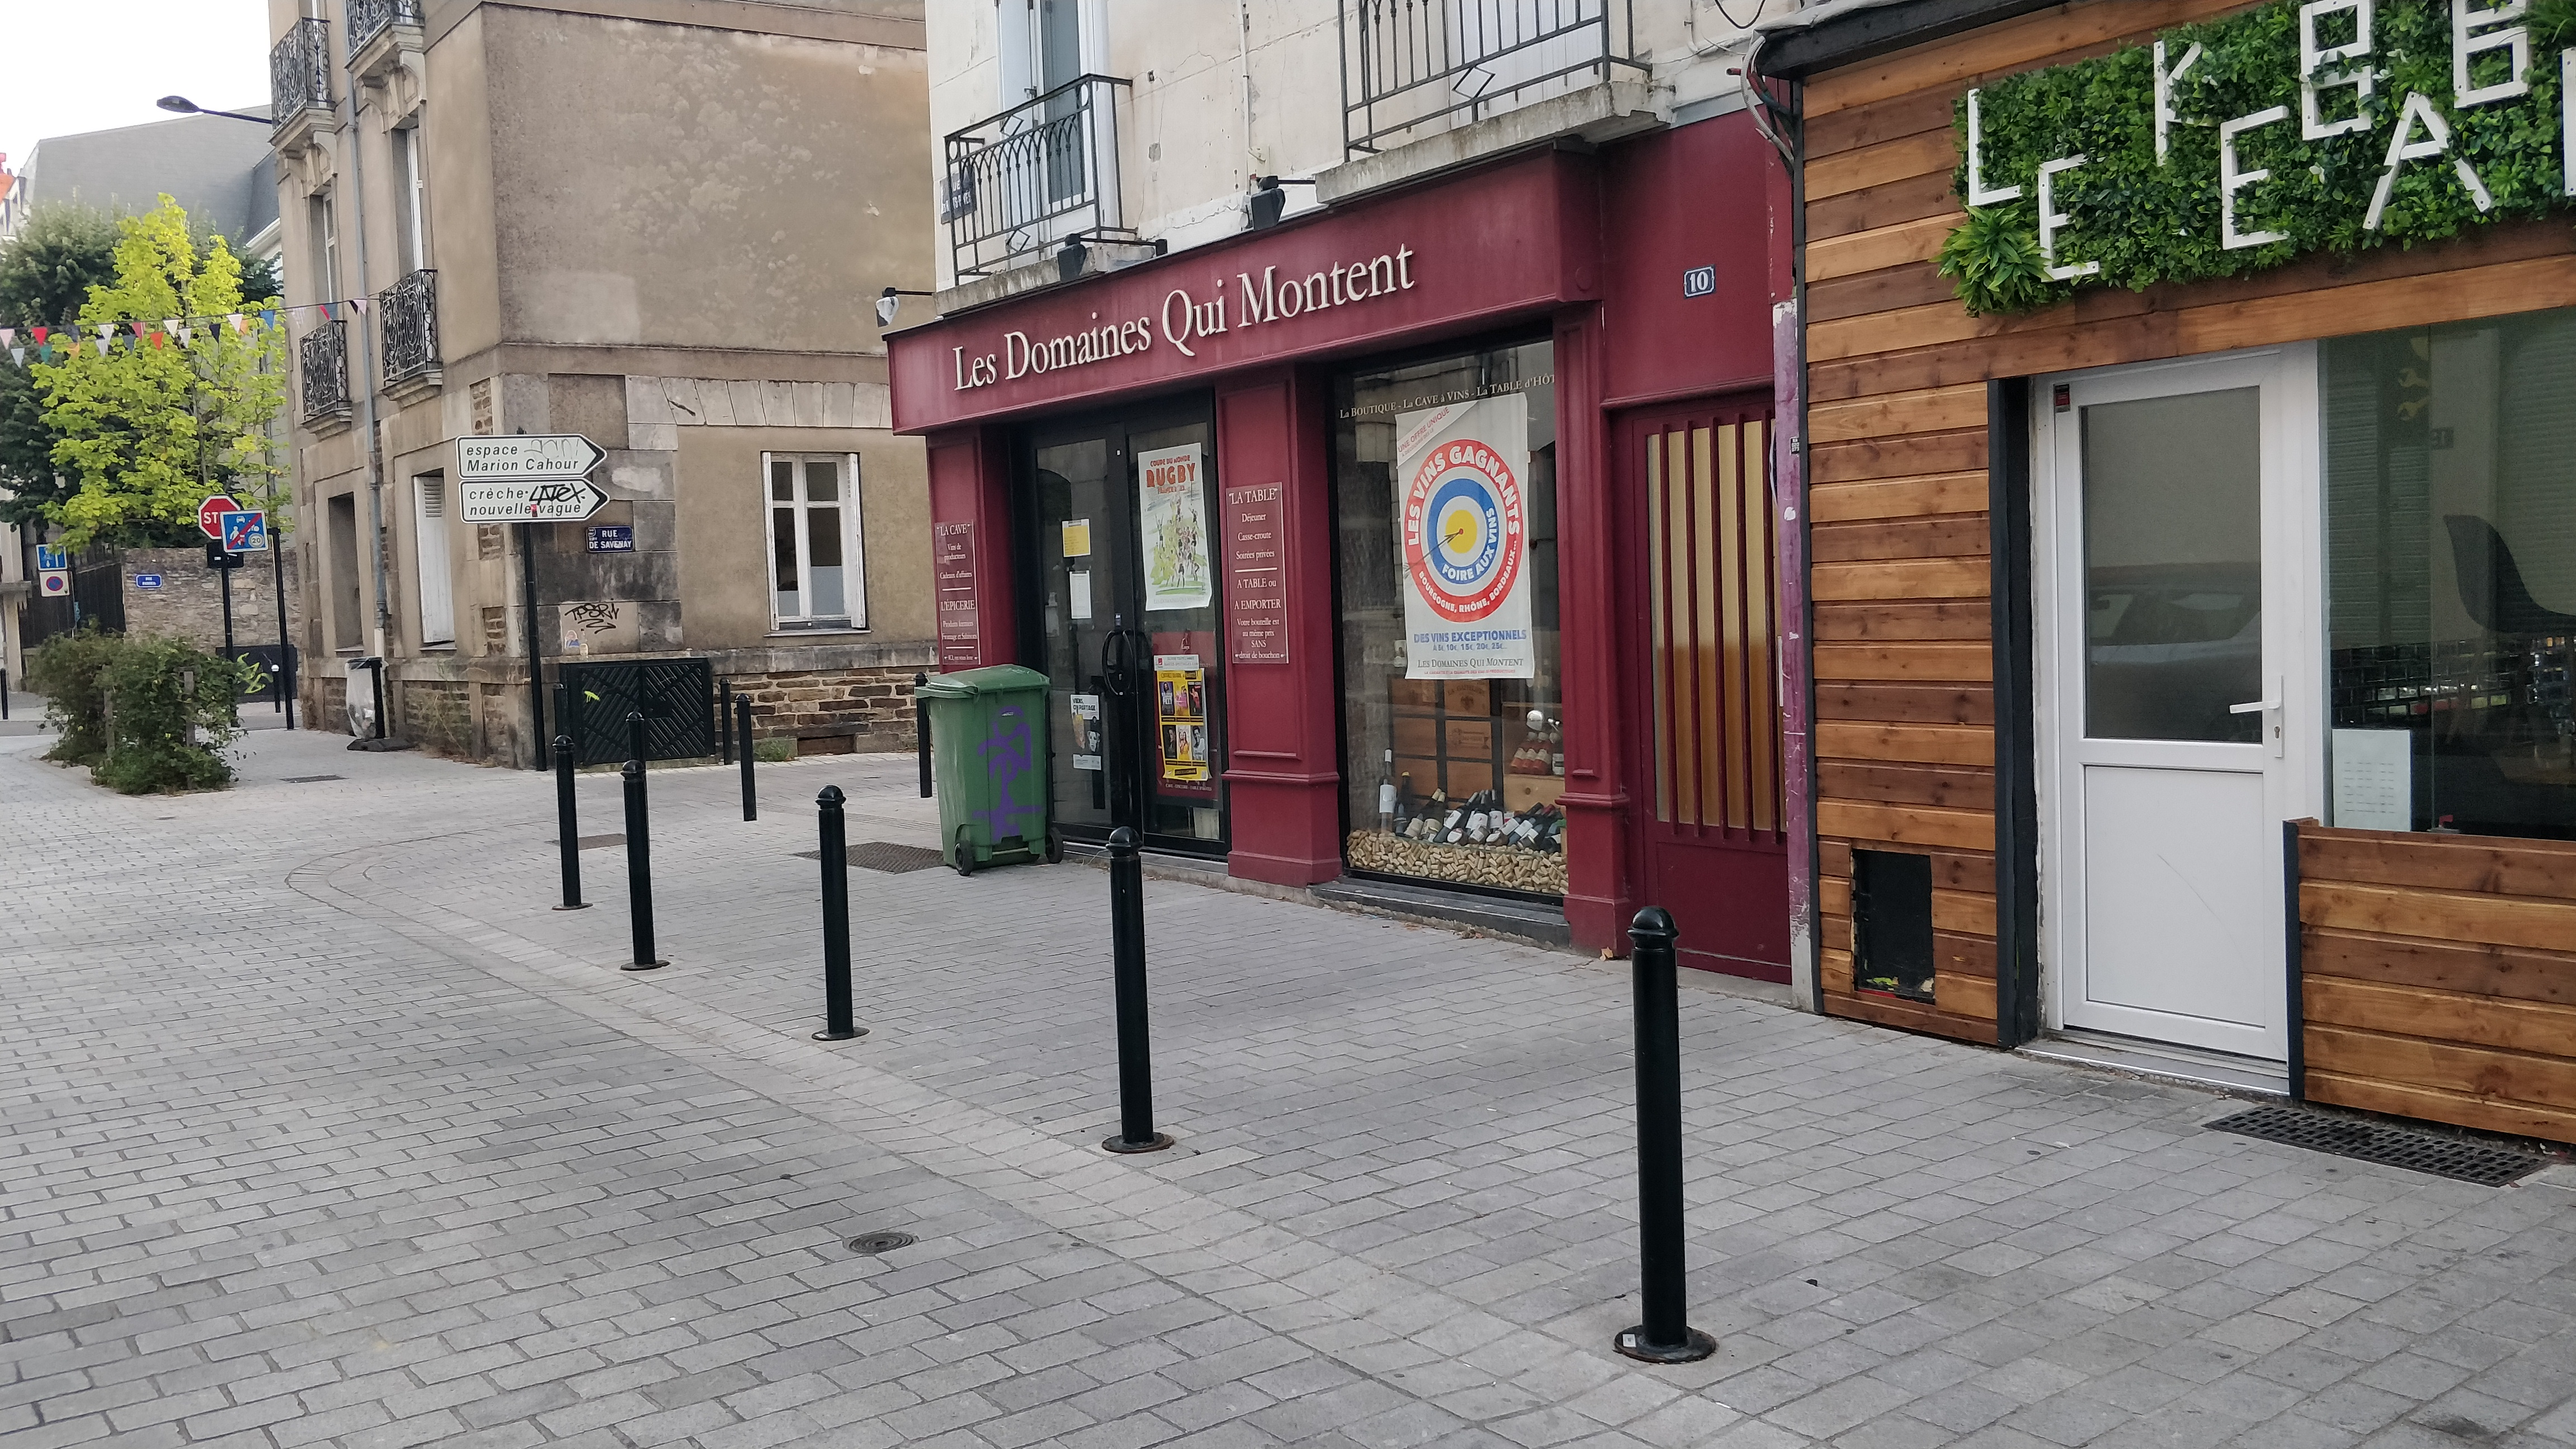
\includegraphics[width=0.7\textwidth]{images/IMG_20230914_075143-ped.jpg}
  \caption{Un trottoir au niveau de la chaussée : cette barrière
    prévient l'accès des voitures tout en garantissant une circulation
    fluide pour les piétons, y compris ceux à mobilité réduite, avec
    des poussettes ou accompagnés de jeunes enfants.}
  \label{fig:ped-flat}
\end{figure}

Malgré les rampes aux passages piétons, les trottoirs restent une
entrave pour beaucoup, surtout pour les personnes à mobilité réduite
et les parents avec poussettes. Leur déplacement est souvent
compliqué, limitant leur autonomie.

Nous plaidons pour une refonte de nos espaces urbains centrée sur
l’accessibilité. Plutôt que des trottoirs surélevés, envisageons des
bornes régulières le long des zones piétonnes (voir
figure~\ref{fig:ped-flat}). Ces bornes, tout en étant accessibles aux
piétons, bloqueraient l'accès aux voitures, garantissant ainsi la
sécurité.

Adopter cette vision c'est choisir une ville plus accessible,
sécurisée, et orientée vers l'humain. Nantes et les Pays de la Loire
doivent saisir cette opportunité pour le bien-être de tous leurs
citoyens.


\chapter{Transports collectifs}

% \textit{Mobilité pour Tous : les transports collectifs comme pilon
%   central de la mobilité métropolitaine}

Si le vélo et la marche sont des moyens de transport économiques et
adaptés à environ la moitié de la population pour de courts trajets de
quelques kilomètres, une autre partie de la population nécessite une
alternative. Que ce soit en raison de l'absence de vélo, de problèmes
de santé, de la préférence pour d'autres modes de transport ou de la
nécessité de parcourir de plus longues distances, tous n'opteront pas
pour la marche ou le vélo. En effet, si la majorité des déplacements
au sein de la Métropole sont courts, la plupart des trajets qui
touchent la métropole dépassent ses frontières et sont plus longs.

Historiquement, nous avons considéré les transports en commun
principalement comme un moyen d'accéder au travail en France, limitant
ainsi leur pertinence en dehors des heures de pointe. Cette
perspective a renforcé l'idée que la voiture reste essentielle pour la
majorité des déplacements.

Percevoir la Métropole et la région comme des vecteurs de mobilité
nous conduit inévitablement à envisager les transports collectifs
comme un service uniformément disponible tout au long de la journée et
de la soirée. Votre voiture part lorsque vous le décidez. Si les
transports en commun ne répondent pas à cette simple exigence, ils ne
pourront jamais prétendre à leur juste place comme une option parmi
d'autres.

Pour que les transports collectifs deviennent véritablement une
solution de mobilité fiable et complète, la refonte de notre approche
est nécessaire pour assurer la disponibilité et l'efficacité des
transports collectifs à tout moment de la journée.


\section{Transitions fluides entre systèmes}

% \textit{Harmonisation des Règles et Réglementations des Transports
%   Publics : Vers une Mobilité Sans Frontières}

Lors de nos déplacements en voiture, nous sommes habitués à
reconnaître les panneaux de signalisation et les règles routières au
fur et à mesure de notre trajet, à emprunter les routes de notre
choix, à faire le plein (essence ou électricité) sans se soucier du
fournisseur, et même à traverser les frontières communales et
nationales en toute simplicité.

Cependant, lorsque nous optons pour les transports en commun, les
règles changent d'une commune à l'autre, d'une région à l’autre. Le
tarif (avec toutes ses complexités locales) doit être payé séparément
et à l'aide d'un instrument différent à chaque fois. Même la
navigation exige souvent l'utilisation d'un nouvel outil à chaque
changement de contrôle administratif.

Afin de permettre aux citoyens de voyager comme bon leur semble, avec
un seul tarif et un unique moyen de paiement, il est impératif que les
agglomérations et les régions collaborent pour harmoniser les règles
et les réglementations entre les différents systèmes de transport
public (incluant les bus, les cars, les trains, les bateaux et les
locations de vélos). Nous devons rapidement évoluer vers un système
similaire à celui des Pays-Bas, de Londres et de Lisbonne (pour citer
trois exemples), qui autorise les utilisateurs même non enregistrés à
voyager en utilisant les instruments de paiement sans contact (carte
bancaire, téléphone) qu'ils possèdent déjà, sans inscription au
préalable.

Cette transition vers un système intégré au niveau des règles
tarifaires et instruments de paiement permettra d'offrir aux usagers
une expérience de déplacement fluide, prévisible et cohérente, tout en
simplifiant les démarches administratives et les modes de paiement.

\refs

\link{https://www.intelligenttransport.com/transport-articles/73782/mobile-ticketing-contactless-payment-germany/}

\link{https://tfl.gov.uk/fares/how-to-pay-and-where-to-buy-tickets-and-oyster/pay-as-you-go/contactless-and-mobile-pay-as-you-go}


\section{Une fréquence crédible}

Les transports collectifs des agglomérations jouent un rôle clé grâce
à la fréquence des passages, à la portée de leur service et à la
cohérence du maillage entre les différentes lignes. Toutefois, pour
certaines lignes, la fréquence de passage est si faible qu'elle
compromet l'efficacité du maillage. De ce fait, l'attrait de ces
lignes se limite aux utilisateurs les plus patients.

Actuellement, de nombreux déplacements matinaux et vespéraux sont
effectués en voiture, principalement parce que les correspondances
entre les différents modes de transport ne sont pas optimisées pour le
confort des voyageurs.

Pour assurer une mobilité fluide et une prévisibilité des trajets, il
est essentiel de garantir une fréquence de passage régulière sur
l'ensemble des lignes tout au long de leur période d'opération.


\section{Redynamiser le TER pour une mobilité crédible}

La mobilité est l'épine dorsale de toute région, toute métropole en
plein essor : les Pays de la Loire, avec Nantes Métropole en son cœur,
n'est pas une exception. Le transport régional (TER et car Aléop) a un
rôle crucial à jouer pour assurer une mobilité durable et efficiente
pour tous. Cependant, à l'heure actuelle, ni le TER ni le car n'est
considéré comme une option de mobilité crédible pour de nombreux
citoyens.

L'un des principaux défis est sa fréquence insuffisante. Pour attirer
plus d'usagers et répondre aux besoins de mobilité croissants, il est
impératif d'augmenter la fréquence des trains. Une plus grande
fréquence réduit les temps d'attente, rendant le voyage en train plus
attrayant par rapport à d'autres modes de transport moins écologiques.

La prévisibilité est la clé de la confiance. Si les citoyens savent
qu'un train passe toutes les 15 minutes, par exemple, ils n'ont pas
besoin de consulter constamment un horaire. Cela leur permet de se
rendre à la gare avec l'assurance qu'ils n'attendront pas
longtemps. Un intervalle uniforme et prévisible, tout au long de la
journée, renforce la crédibilité du TER et du car comme moyen de
transport fiable, réduisant ainsi la nécessité du recours à la
voiture.

Une véritable option de transport doit être disponible lorsque les
gens en ont besoin. Le TER et le car doivent fonctionner tôt le matin
pour ceux qui commencent leur journée avant l'aube et continuer tard
le soir pour ceux qui rentrent après une longue journée ou une sortie
vespérale. En élargissant l'amplitude des heures de fonctionnement,
nous assurons que le train est une option de mobilité viable et
crédible, quel que soit le moment de la journée.

Un objectif minimal doit être un cadencement toutes les 15 minutes
toute la journée à l'exception des petites heures de la nuit.


\section{De nouvelles lignes}

Au cours de ces cinquante dernières années, nous avons progressivement
abandonné les lignes de train régionales en France. Un réseau jadis
bien connecté s'est réduit au point que nous évoquons l'expression «
étoile ferroviaire » à Nantes sans percevoir l'ironie qu'elle
renferme, car il ne reste en réalité que cela.

Le rail constitue l'épine dorsale idéale d'un système de transport
public.

Il est impératif de rouvrir les lignes ferroviaires là où cela reste
possible. Plusieurs exemples se présentent, tels que l'Île de Nantes
(la
\href{https://www.mobilitains.fr/tb/t/ligne-johanna-rolland-2021/}{Ligne
  Johanna Rolland}) et les lignes en direction du Pellerin, de
Paimbœuf, de Grand Lieu et de Carquefou, ainsi que la ligne
Saint-Nazaire - Redon.

Deuxièmement, il nous faut examiner où de nouvelles lignes ou des
lignes renforcées seraient pertinentes. Nombre de nos lignes ne
comportent qu'une voie unique sans possibilité de dépassement. Le jour
où nous souhaiterons augmenter le service, nous serions confrontés à
un délai de 15 ans en raison du simple besoin de construire des zones
de dépassement et des systèmes de signalisation capables de les
utiliser efficacement.

\begin{figure}[ht]
  \centering
  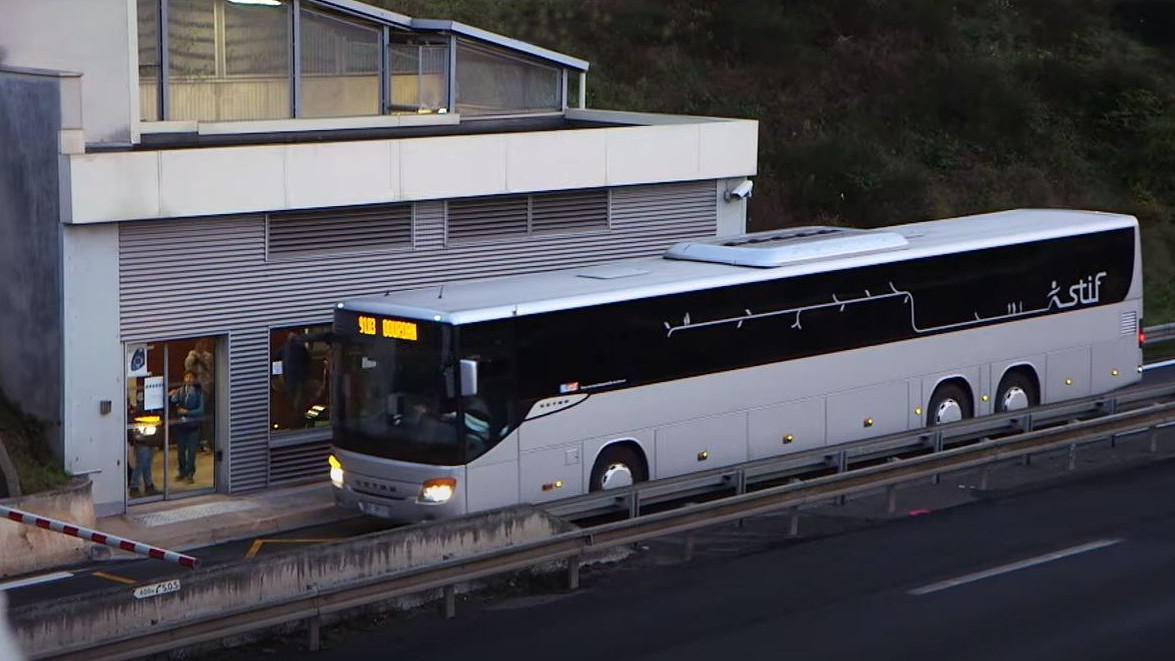
\includegraphics[width=0.7\textwidth]{images/car-express.jpg}
  \caption{Station de car express en Île-de-France : le car ne dévie
    pas de sa voie principale, il emprunte une voie d'arrêt dédiée
    pour l'embarquement et le débarquement des passagers. Sur le plan
    architectural, nul doute que nous pourrions faire preuve d'un peu
    plus d'élégance.}
  \label{fig:car-express}
\end{figure}

Troisièmement, il est primordial de mettre en place des services de
cars express. Contrairement à notre système actuel de cars qui relie
cheminement de village en village, les cars express disposeraient de
stations dédiées sur nos autoroutes et voies rapides, dotées
d'infrastructures sécurisées pour les cyclistes et les piétons, ainsi
que de parkings vélo et voiture afin de ne pas dépendre de la
voiture. Les stations seraient espacées d'environ 5 km les unes des
autres, de manière à ce que chacun qui le souhaite puisse facilement
rejoindre une station de car express en vélo. Les cars ne quitteraient
pas sa route, mais entreraient simplement dans une courte voie de
chargement. De cette manière, les cars express pourraient concurrencer
efficacement les voitures. De tels systèmes peuvent être mis en place
en seulement quelques années, les options ferroviaires suivant là où
le trafic le justifie.

\refs

\textit{Transports : les oubliés de la République: Quand la route reconnecte le territoire}, André Broto, 2022.


\section{De nouvelles gares}

La saturation progressive de la gare de Nantes n’est plus un sujet de
conjecture, mais une réalité à laquelle nous sommes
confrontés. L’importance de la mobilité urbaine exige une réflexion en
profondeur. Ainsi, nous préconisons la création de cinq nouvelles
gares pour désengorger la gare principale et offrir une meilleure
accessibilité.

Malgré les travaux de réaménagement de l'Île de Nantes, ces quartiers
de la ville ne sont pas desservis par d'autres moyens de transport
régional que la voiture individuelle. Il est donc crucial d'adresser
cette insuffisance en intégrant deux nouvelles gares à la ligne
existante et en prolongeant le tronçon restant de la
\href{https://www.mobilitains.fr/tb/t/ligne-johanna-rolland-2021/}{Ligne
  Johanna Rolland} jusqu'au CHU et à l'extrémité de l'île. Cette
extension mènerait à la nouvelle gare des Antilles et comprendrait un
franchissement de la Loire en direction de Chantenay.

\textbf{Médiathèque.} Les travaux du tunnel entre la gare centrale et
Chantenay, très probables dans les dix à vingt prochaines années dus à
l'affaissement lent des caissons dans un sol sableux, est une
opportunité unique. Rétablir la gare de la Bourse en souterrain, et la
mettre en correspondance avec l'arrêt tramway de la Médiathèque,
garantirait une meilleure fluidité des mouvements de passagers en
évitant que tout passager pour Nantes doit changer à la gare centrale.

\textbf{Beaulieu.}
L'extension en cours du centre commercial Beaulieu, d'une superficie
de 5000 mètres carrés, met en évidence l'importance de la mobilité
dans cette zone. Cependant, la création de nouvelles places de
stationnement pour voitures ne répond pas de manière adéquate à cette
exigence. La ligne de TER qui longe cette zone doit être mise à
contribution en créant une gare de Beaulieu, stimulant ainsi la
mobilité durable et minimisant la dépendance à la voiture
individuelle.  Ce serait également le bienvenu pour les commerçants
qui verraient un trafic supplémentaire grâce aux voyageurs en train.

\textbf{Mangin.}
Bien que souvent envisagée en conjonction avec Beaulieu, Mangin a
toutes les raisons d'avoir sa propre station. La distance entre
Beaulieu et Mangin, supérieure à un kilomètre, justifie cette
distinction. D’ailleurs, tous les trains n'ont pas besoin de s'arrêter
dans ces deux gares, même si la fréquence actuelle des trains rend
difficilement imaginable une alternance. Les exemples, comme celui du
RER C à Paris, réfutent l'idée selon laquelle deux gares ne peuvent
coexister à une distance de marche de 15 minutes.

\textbf{CHU.}
Le nouveau CHU, générateur de plus de 20,000 emplois, et attirant
chaque jour de nombreux patients et visiteurs, nécessite une liaison
ferroviaire régionale. L'espace permettant une desserte depuis le nord
et le sud est toujours disponible. Si le tramway en cours de
construction est une avancée pour les Nantais, il ne répond pas
entièrement aux besoins de ceux venant de régions éloignées, qui
pourraient ainsi délaisser leur voiture.

\textbf{La gare des Antilles et son pont.}  Desservir l’extrémité de
l'Île de Nantes renforcera la cohérence du réseau. Un franchissement
de la Loire (le pont des Antilles, proposé) pour rejoindre la gare de
Chantenay et les lignes en direction de Saint Nazaire, Le Croisic,
Redon, et la Bretagne, est un levier stratégique. Cela allègerait
considérablement la sollicitation de la gare centrale de Nantes,
évitant que tous les trains y transitent.  De plus, en cas de travaux
ou d'incident dans le tunnel entre Chantenay et la gare centrale de
Nantes, une telle alternative préserverait la connectivité entre
Nantes, l'ouest et le nord.

% https://www.20minutes.fr/nantes/3181159-20211124-nantes-centre-commercial-beaulieu-etend-recevoir-primark

% https://actu.fr/pays-de-la-loire/nantes_44109/nantes-pourquoi-y-a-t-il-des-travaux-pres-du-centre-commercial-beaulieu_41278110.html


\section{La gare centrale de Nantes}

La gare centrale de Nantes, point névralgique du réseau ferroviaire de
la région Pays de la Loire, connaît une affluence sans précédent
récent. Cette croissance reflète la vitalité de la région, mais elle
pose également un ensemble de défis majeurs en termes d'aménagement,
de logistique et de mobilité.

La première réponse à cette affluence est d'assurer une circulation
fluide et sécurisée des voyageurs. Pour ce faire, il est impératif de
penser à l'espace autrement. La mise en place d'un passage surélevé à
l'extrémité est des quais est une solution viable. Ce passage
faciliterait non seulement le flux de voyageurs entre les différentes
voies, mais créerait également un lien direct avec la station de
tramway de Manufacture au nord et avec le nouveau quartier d'Europe au
sud.

En reliant la gare au quartier d'Europe et à la station de tramway
(sans construction de parking voiture supplémentaire), nous
permettrons aux voyageurs d'accéder facilement à la gare depuis
différentes parties de la ville. Cette connectivité améliorée
favoriserait une transition fluide entre les différents modes de
transport, contribuant ainsi à réduire la congestion routière et les
émissions de carbone.

Une deuxième réponse et enjeu majeur concerne la logistique des trains
eux-mêmes. La gare centrale ne doit plus être considérée uniquement
comme un point de terminaison pour tous les trains. En effet, une
grande partie des trains régionaux pourrait continuer leur trajet vers
une autre destination. Même les trains longue distance pourraient
continuer leur trajet au moins jusqu'à Chantenay. Cette continuité
présente plusieurs avantages : elle fluidifie le trafic, évite les
engorgements dans les voies de garage et permet une meilleure gestion
de l'espace ferroviaire.


\section{L'accès pédestre et cycliste aux transports collectifs}

Pour parvenir à une augmentation de la fréquence et de l'amplitude du
service de transport public, il est primordial d'accroître l'accès à
ces services. Aujourd'hui, une grande partie de la population accède
aux services de transport en commun en voiture. Cette pratique n'est
ni durable ni écologiquement souhaitable.

Un des principaux obstacles est l'accès aux transports publics à pied
ou à vélo. Face à ce défi, il est impératif de garantir que chaque
arrêt de bus, tramway, et car ainsi que toute gare ferroviaire soit
accessible en toute sécurité en dix minutes à pied (soit une distance
d'environ 500 mètres) et à vélo (soit une distance d'environ 3 km).

Cependant, assurer une bonne accessibilité n'est qu'une partie de la
solution. Il est également essentiel de fournir des installations de
stationnement adaptées pour les vélos. Le caractère "adéquat" de ces
installations peut varier selon la localité. Dans les zones urbaines,
où les contraintes sont plus marquées en raison de la densité et des
risques de vol, le besoin en matière de sécurité et de protection
contre les intempéries est plus élevé.

À l'inverse, dans les zones rurales, les exigences sont souvent moins
strictes. Une simple attache ou appui, éventuellement couverte d'un
toit pour le protéger de la pluie, suffirait généralement.


\section{Harmonisation du matériel roulant}

La région de Nantes, avec son dynamisme économique et démographique,
mérite une attention toute particulière en ce qui concerne sa
mobilité. Deux des lignes majeures, Nantes-Clisson (inaugurée en tant
que tram-train le 15 juin 2011) et Nantes-Châteaubriant (ouverte le 24
février 2014), ont adopté du matériel roulant spécifique, différent du
reste du système ferroviaire français. Cette décision, quoique basée
sur des raisons politiques, économiques, et contextuelles, a des
répercussions significatives sur la mobilité de la région.

\begin{figure}[ht]
  \centering
  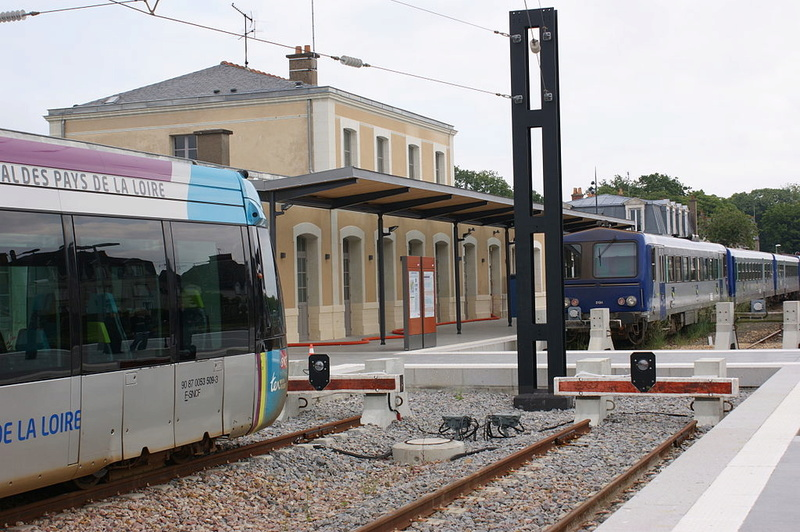
\includegraphics[width=0.7\textwidth]{images/gare-chateaubriant-1.jpg}
  \caption{À la gare de Châteaubriant, divers matériels roulants
    présentent des besoins électriques et de signalisation
    incompatibles, compromettant la liaison entre les régions de
    Nantes et Rennes.}
  \label{fig:chateaubriant}
\end{figure}

Actuellement, la SNCF, ou son futur concessionnaire (également la
SNCF), se trouve dans l'obligation de gérer l'exploitation,
l'entretien et la maintenance de deux systèmes distincts, doublant
ainsi les efforts en termes de ressources humaines et
financières. Cette hétérogénéité du matériel roulant empêche une
fluidité opérationnelle. Par exemple, une liaison directe entre Nantes
et Rennes via Châteaubriant est entravée à cause de l'incompatibilité
technique (voir figure~\ref{fig:chateaubriant}). Les gares intermédiaires
subissent également cette décision, ne permettant pas aux TER
traditionnels de s'arrêter, comme c'est le cas à Savenay.

De surcroît, les infrastructures actuelles, notamment la hauteur des
quais, ne sont pas adaptées aux TER traditionnels. C'est la raison
pour laquelle les tram-trains de Clisson stationnent en périphérie de
la gare de Nantes (voir figure~\ref{fig:clisson}) et que des travaux
d'ajustement ont dû être réalisés sur les quais de la ligne
Nantes-Clisson.

\begin{figure}[ht]
  \centering
  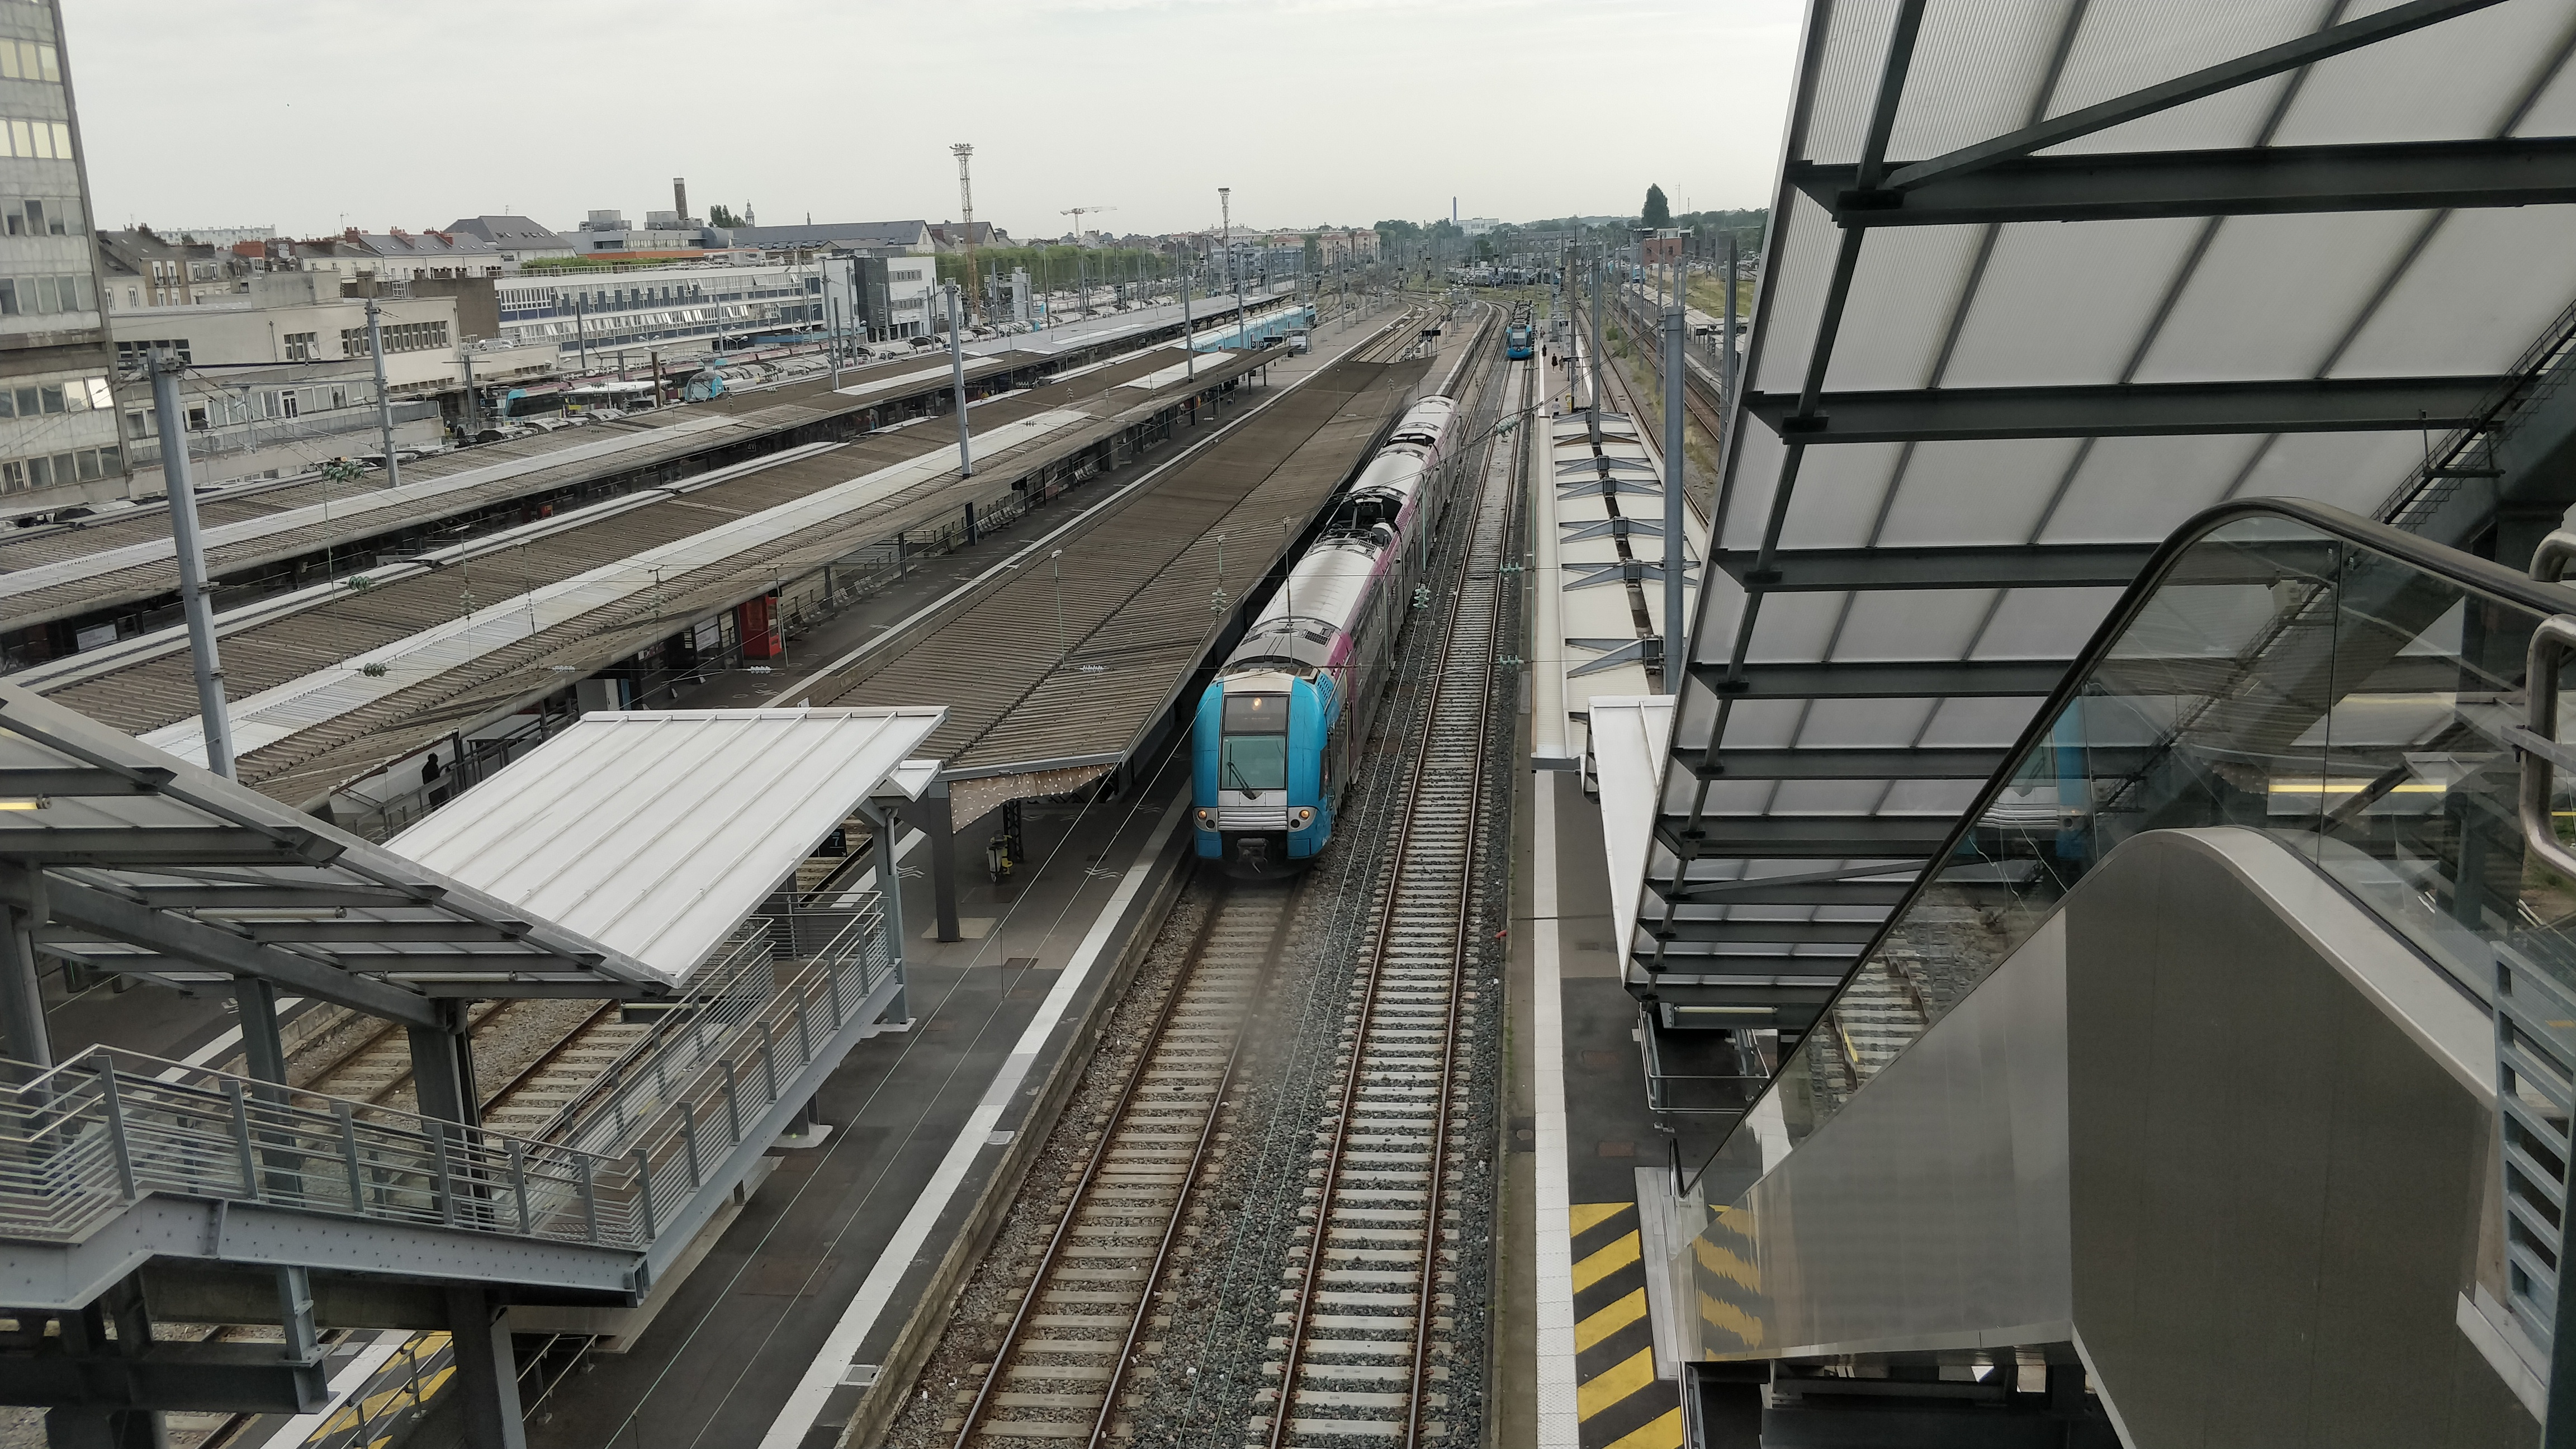
\includegraphics[width=0.7\textwidth]{images/IMG_20230908_104847-clisson.jpg}
  \caption{En premier plan sur la voie de gauche : un TER
    traditionnel.  À l'arrière-plan sur la voie de droite, bien plus
    éloigné et à peine visible, le train-tram en direction de Clisson.
    Si combiner le train et la marche représente une forme de
    multimodalité, ce n'est pas nécessairement la vision typique que
    l'on en a.}
  \label{fig:clisson}
\end{figure}

Concernant les vitesses, il est à noter que les tram-trains ne
dépassent pas 100 km/h, et cette vitesse est encore plus réduite à 30
km/h en zone métropolitaine entre Nantes et
La~Chapelle-sur-Erdre. Ainsi, ils ne peuvent rivaliser avec les
véhicules personnels en termes de rapidité, rendant le choix du train
moins attractif pour beaucoup de trajets.

Le matériel roulant sur ces deux lignes approche les 15 ans depuis son
acquisition par la région (commandé le 25 avril 2007) avec 12 ans en
exploitation. Il est crédible de parler de son renouvellement pour
2050.

Devant ces constats, la nécessité d'harmoniser le matériel roulant
devient impérative pour optimiser l'exploitation ferroviaire. Une
telle démarche permettrait une meilleure desserte pour les habitants
de Nantes et de la région Pays de la Loire, tout en rationalisant les
coûts d'exploitation et de maintenance.

\refs

\begin{itemize}
\item L’échec très discret du tram‐train Nantes‐Châteaubriant\\
\link{https://www.mediacites.fr/enquete/nantes/2017/09/20/lechec-tres-discret-du-tram-train-nantes-chateaubriant/}
\item TRIBUNE – Un avenir pour la ligne Rennes‐Châteaubriant‐Nantes\\
\link{https://www.mediacites.fr/forum/nantes/2017/09/21/un-avenir-pour-la-ligne-rennes-chateaubriant-nantes/}
\item Tram‐train Nantes‐Châteaubriant : quand la Région s’en prend à \dots la Région\\
\link{https://www.mediacites.fr/complement-denquete/nantes/2017/12/07/tram-train-nantes-chateaubriant\%e2\%80\%af-quand-la-region-sen-prend-a-la-region/}
\item Nantes‐Châteaubriant : l’avenir de plus en plus incertain du tram‐train
\link{https://www.mediacites.fr/complement-denquete/nantes/2018/11/15/nantes-chateaubriant-lavenir-de-plus-en-plus-incertain-du-tram-train/}
\item Le tram‐train Nantes – Châteaubriant patine toujours
\link{https://www.mediacites.fr/breve/nantes/2021/01/07/le-tram-train-nantes-chateaubriant-patine-toujours/}
\item Tram‐train Nantes‐Châteaubriant : (encore) 1,5 million d’euros de travaux avant l’ouverture à la concurrence
\link{https://www.mediacites.fr/breve/nantes/2021/12/16/tram-train-nantes-chateaubriant-encore-15-million-deuros-de-travaux-avant-louverture-a-la-concurrence/}
\end{itemize}


\section{Intégration fluide du vélo, train et car}

Le vélo, plus qu'une simple activité sportive, est devenu un élément
central de la mobilité contemporaine. Dans ce contexte, il est crucial
de repenser nos services TER et de transport par car pour qu'ils
répondent aux besoins diversifiés des cyclistes, reflétant par la même
occasion les évolutions sociétales en matière de déplacement.

\begin{figure}[ht]
  \centering
  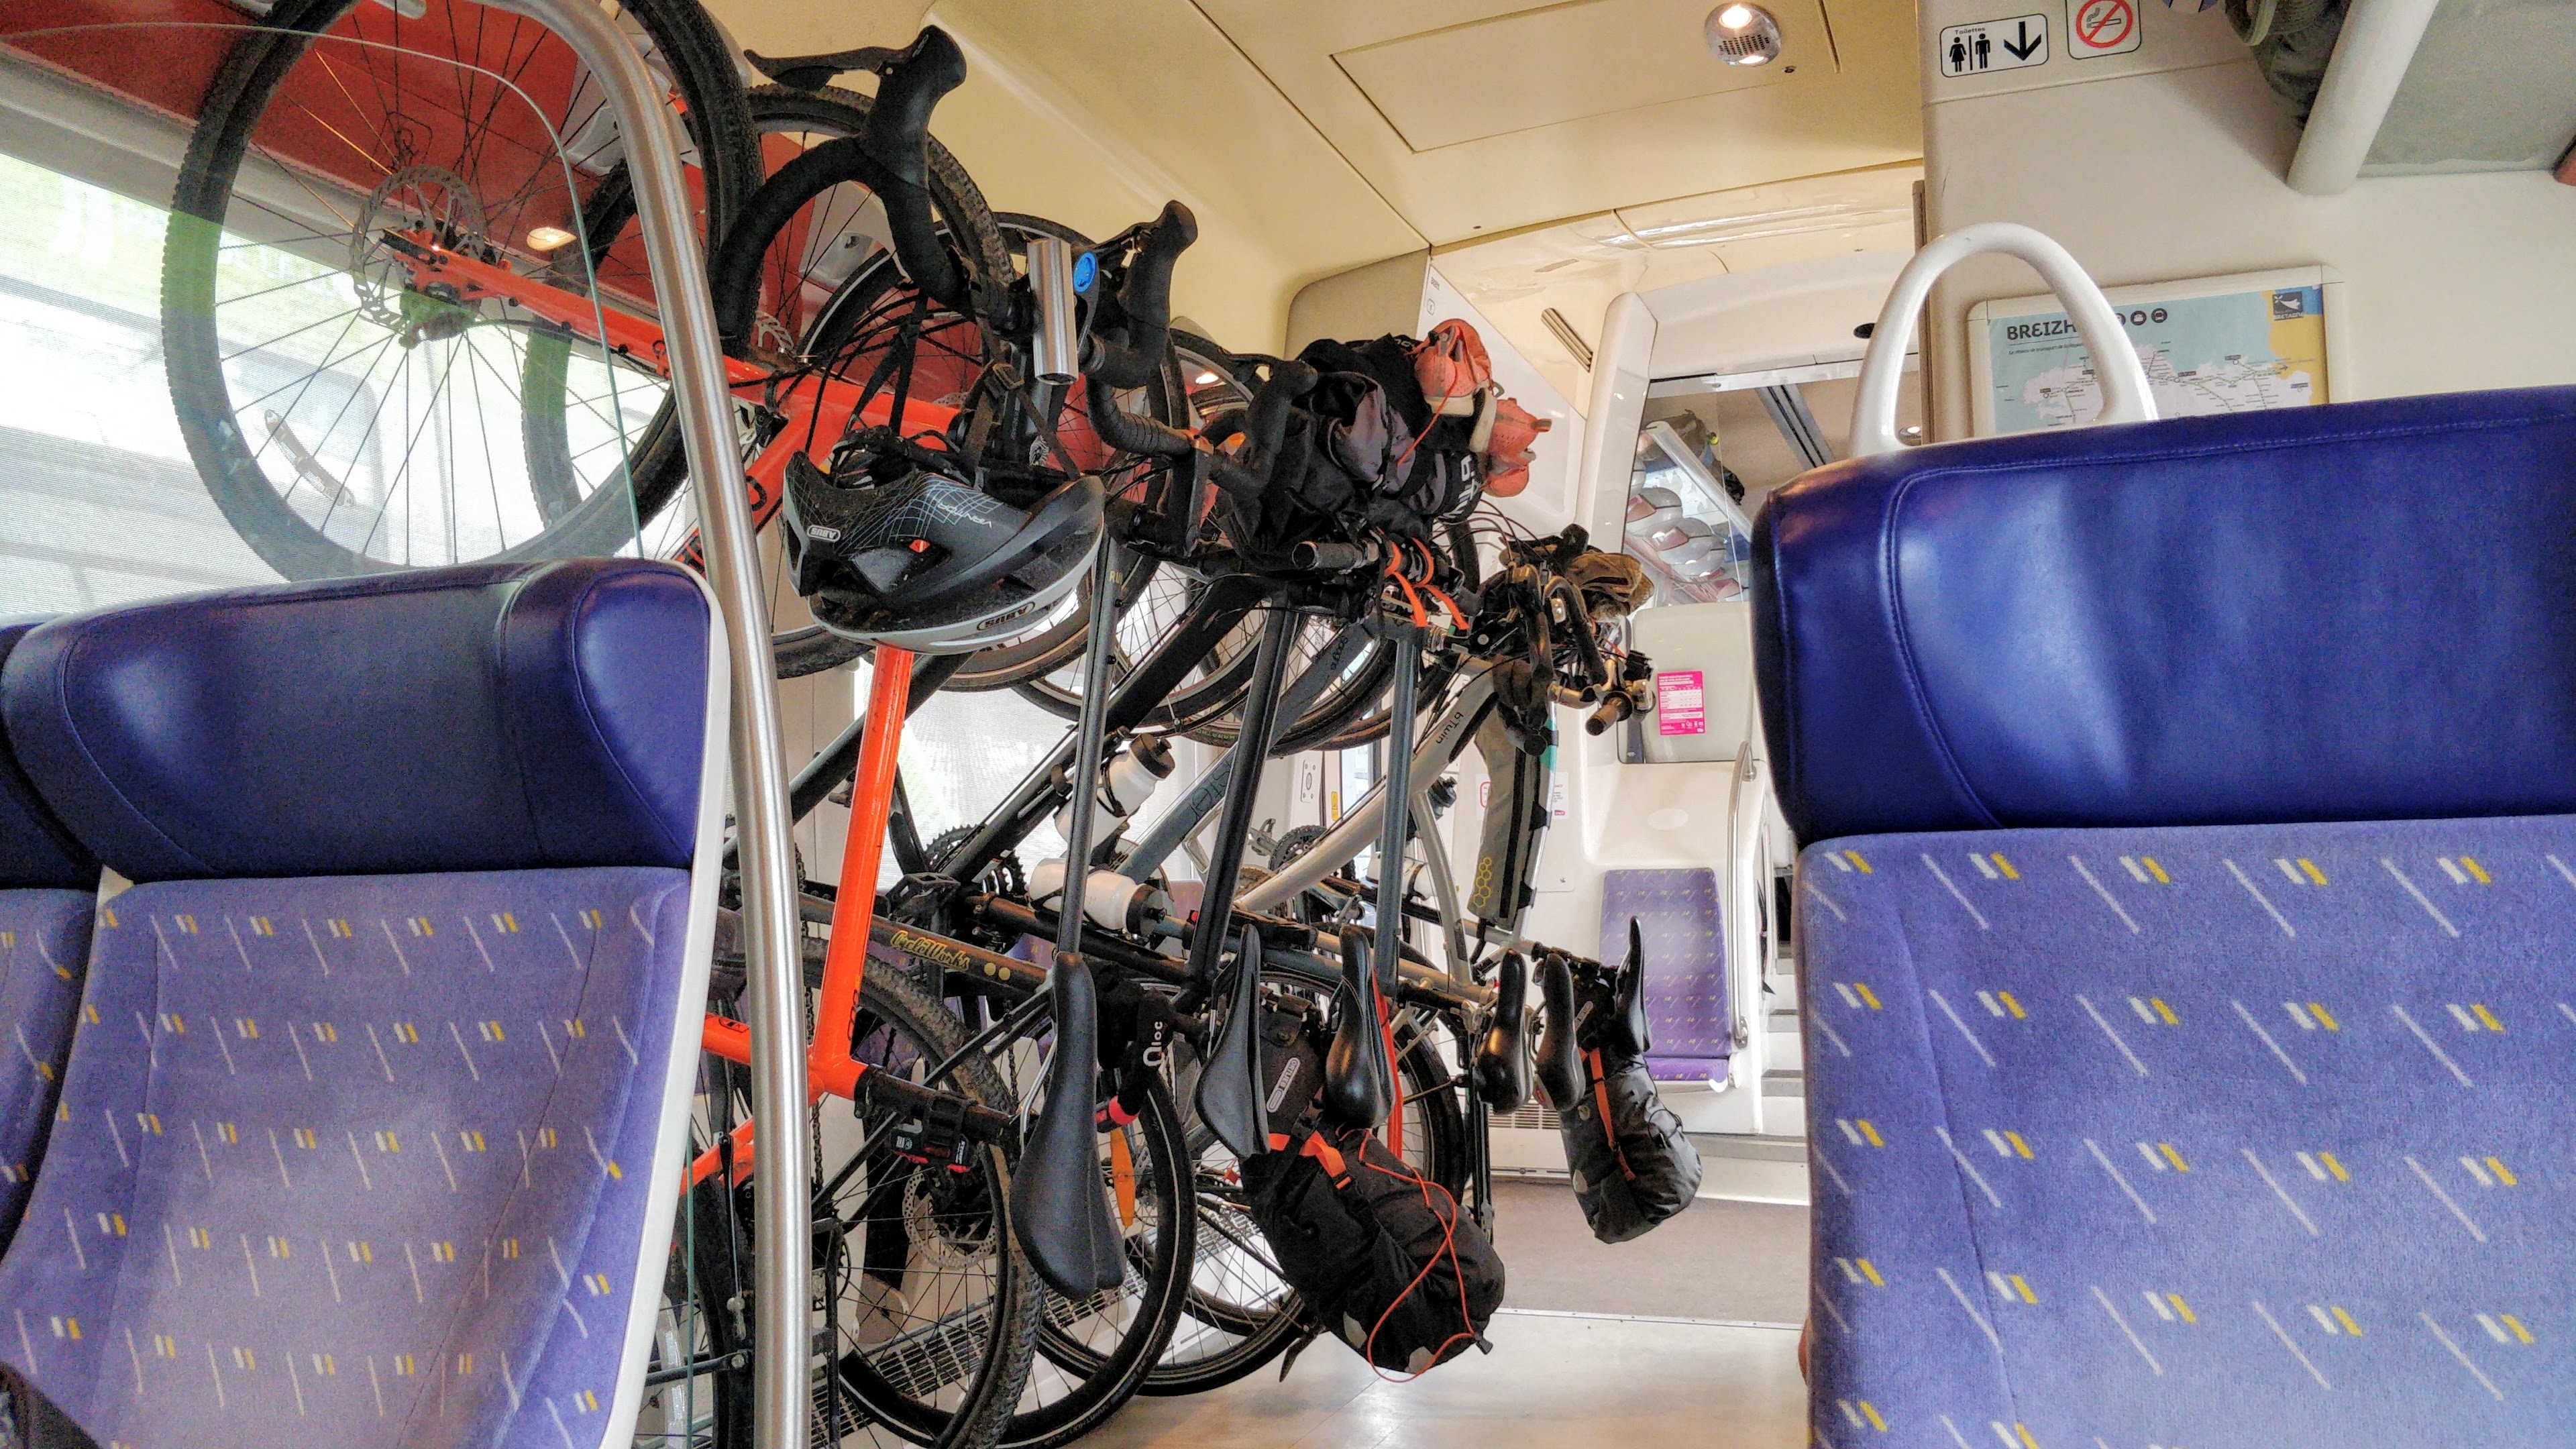
\includegraphics[width=0.7\textwidth]{images/IMG-20220729-WA0001-TER-hanging.jpeg}
  \caption{Cessons de préconiser le rangement vertical des vélos :
    cette idée découle d'une perception naïve où tous les cyclistes
    sont sportifs dotés de vélos légers. Dans un monde visant à
    optimiser la mobilité, nombreux sont les cyclistes qui sont
    jeunes, âgés, ou n'ont pas autant de force physique, et utilisent
    des vélos à assistance électrique ou équipés de sacoches.  De
    plus, ranger un vélo horizontalement facilite la montée et la
    descente des trains, contrairement au rangement vertical.}
  \label{fig:train-velo-vertical}
\end{figure}

Aujourd'hui, la bicyclette n'est plus cantonnée à une utilisation
sportive ou récréative. Elle est un outil quotidien pour de nombreux
citoyens, indépendamment de leur âge, pour leurs déplacements
professionnels ou personnels. Pourtant, nos TER semblent encore pensés
pour des cyclistes sportifs avec vélos légers et sans bagages (voir
figure~\ref{fig:train-velo-vertical}). Quant à nos cars,
l'embarquement de vélos y est souvent complexe, voire inexistant. Une
telle vision ne capture pas l'essence de la mobilité actuelle.

Il est donc urgent d'entamer une transformation radicale de nos TER et
de notre service de cars pour intégrer de manière efficace et pratique
les vélos. Imaginons un système de rangement horizontal (voir
figure~\ref{fig:train-velo-francais-horizontal}), ``roll-on,
roll-off'', où l'on pourrait monter et descendre aisément avec son
vélo, qu'il soit traditionnel ou à assistance électrique, avec ou sans
bagages.

\begin{figure}[ht]
  \centering
  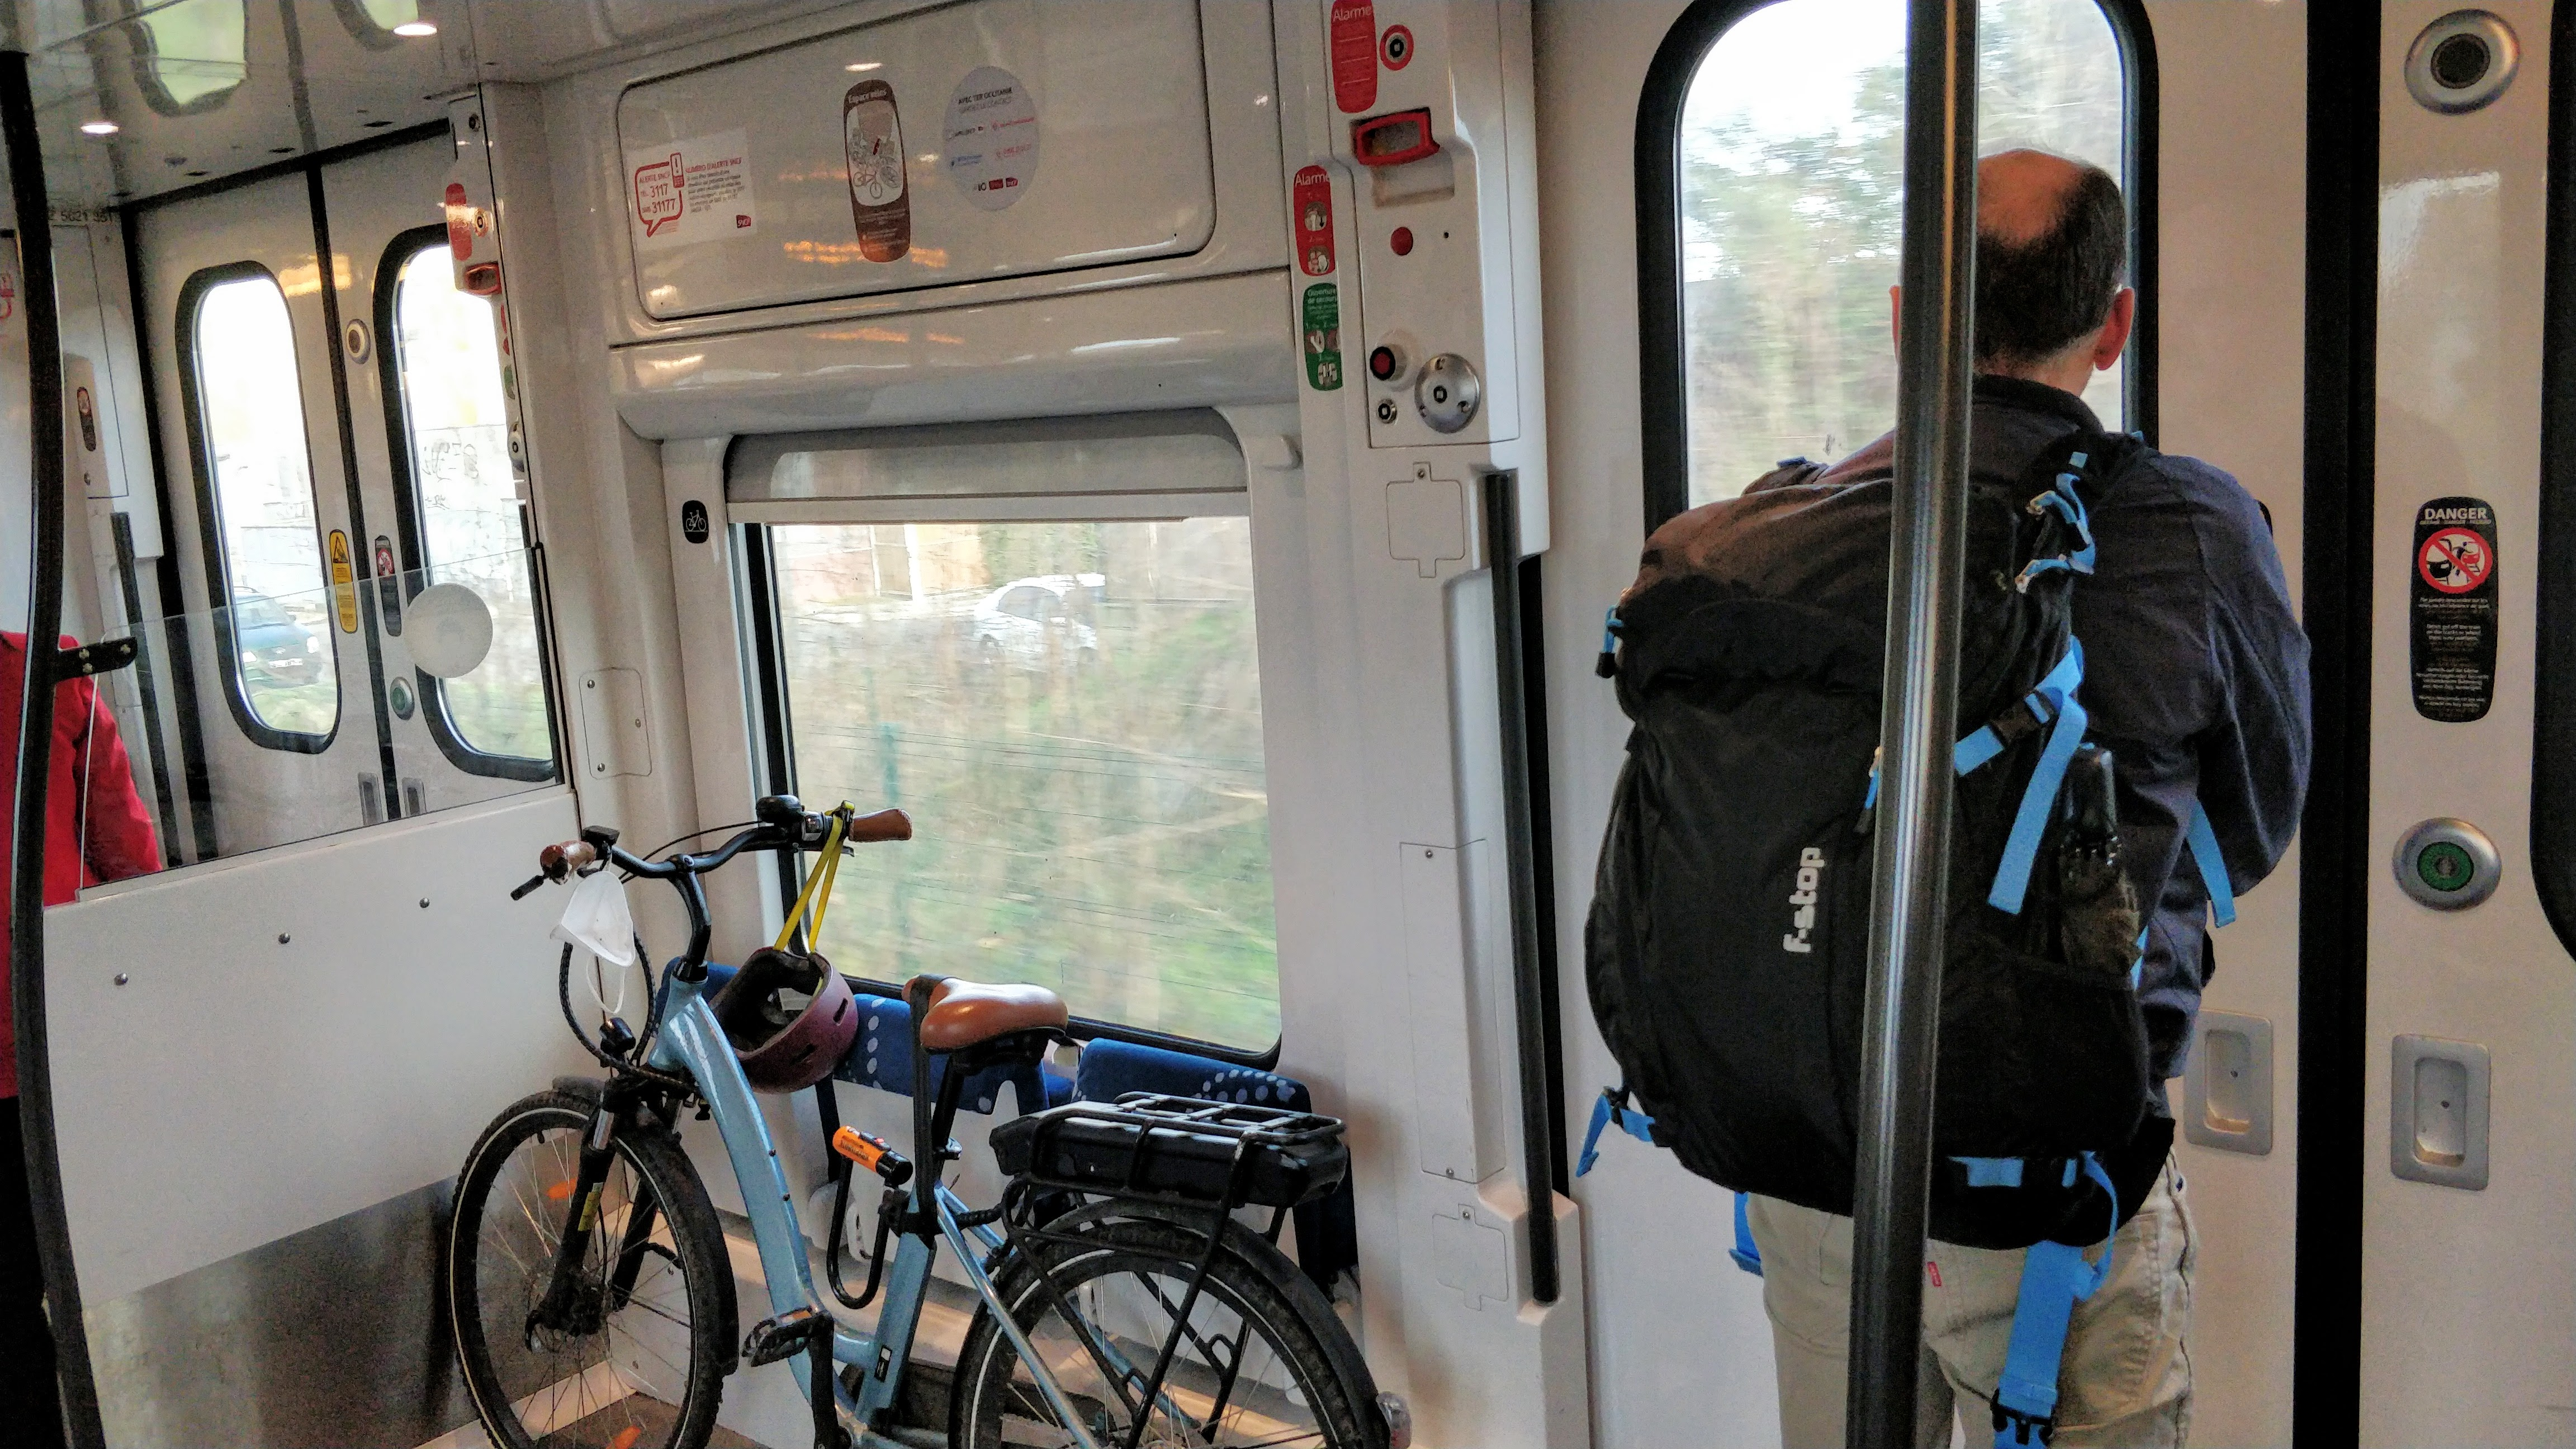
\includegraphics[width=0.7\textwidth]{images/IMG_20221223_145849-TER-horizontal.jpg}
  \caption{Des sièges pliants et polyvalents à bord d'un train
    français avec vélo rangé en horizontal.  Cet espace vélo suffit
    pour trois vélos.}
  \label{fig:train-velo-francais-horizontal}
\end{figure}

\begin{figure}[ht]
  \centering
  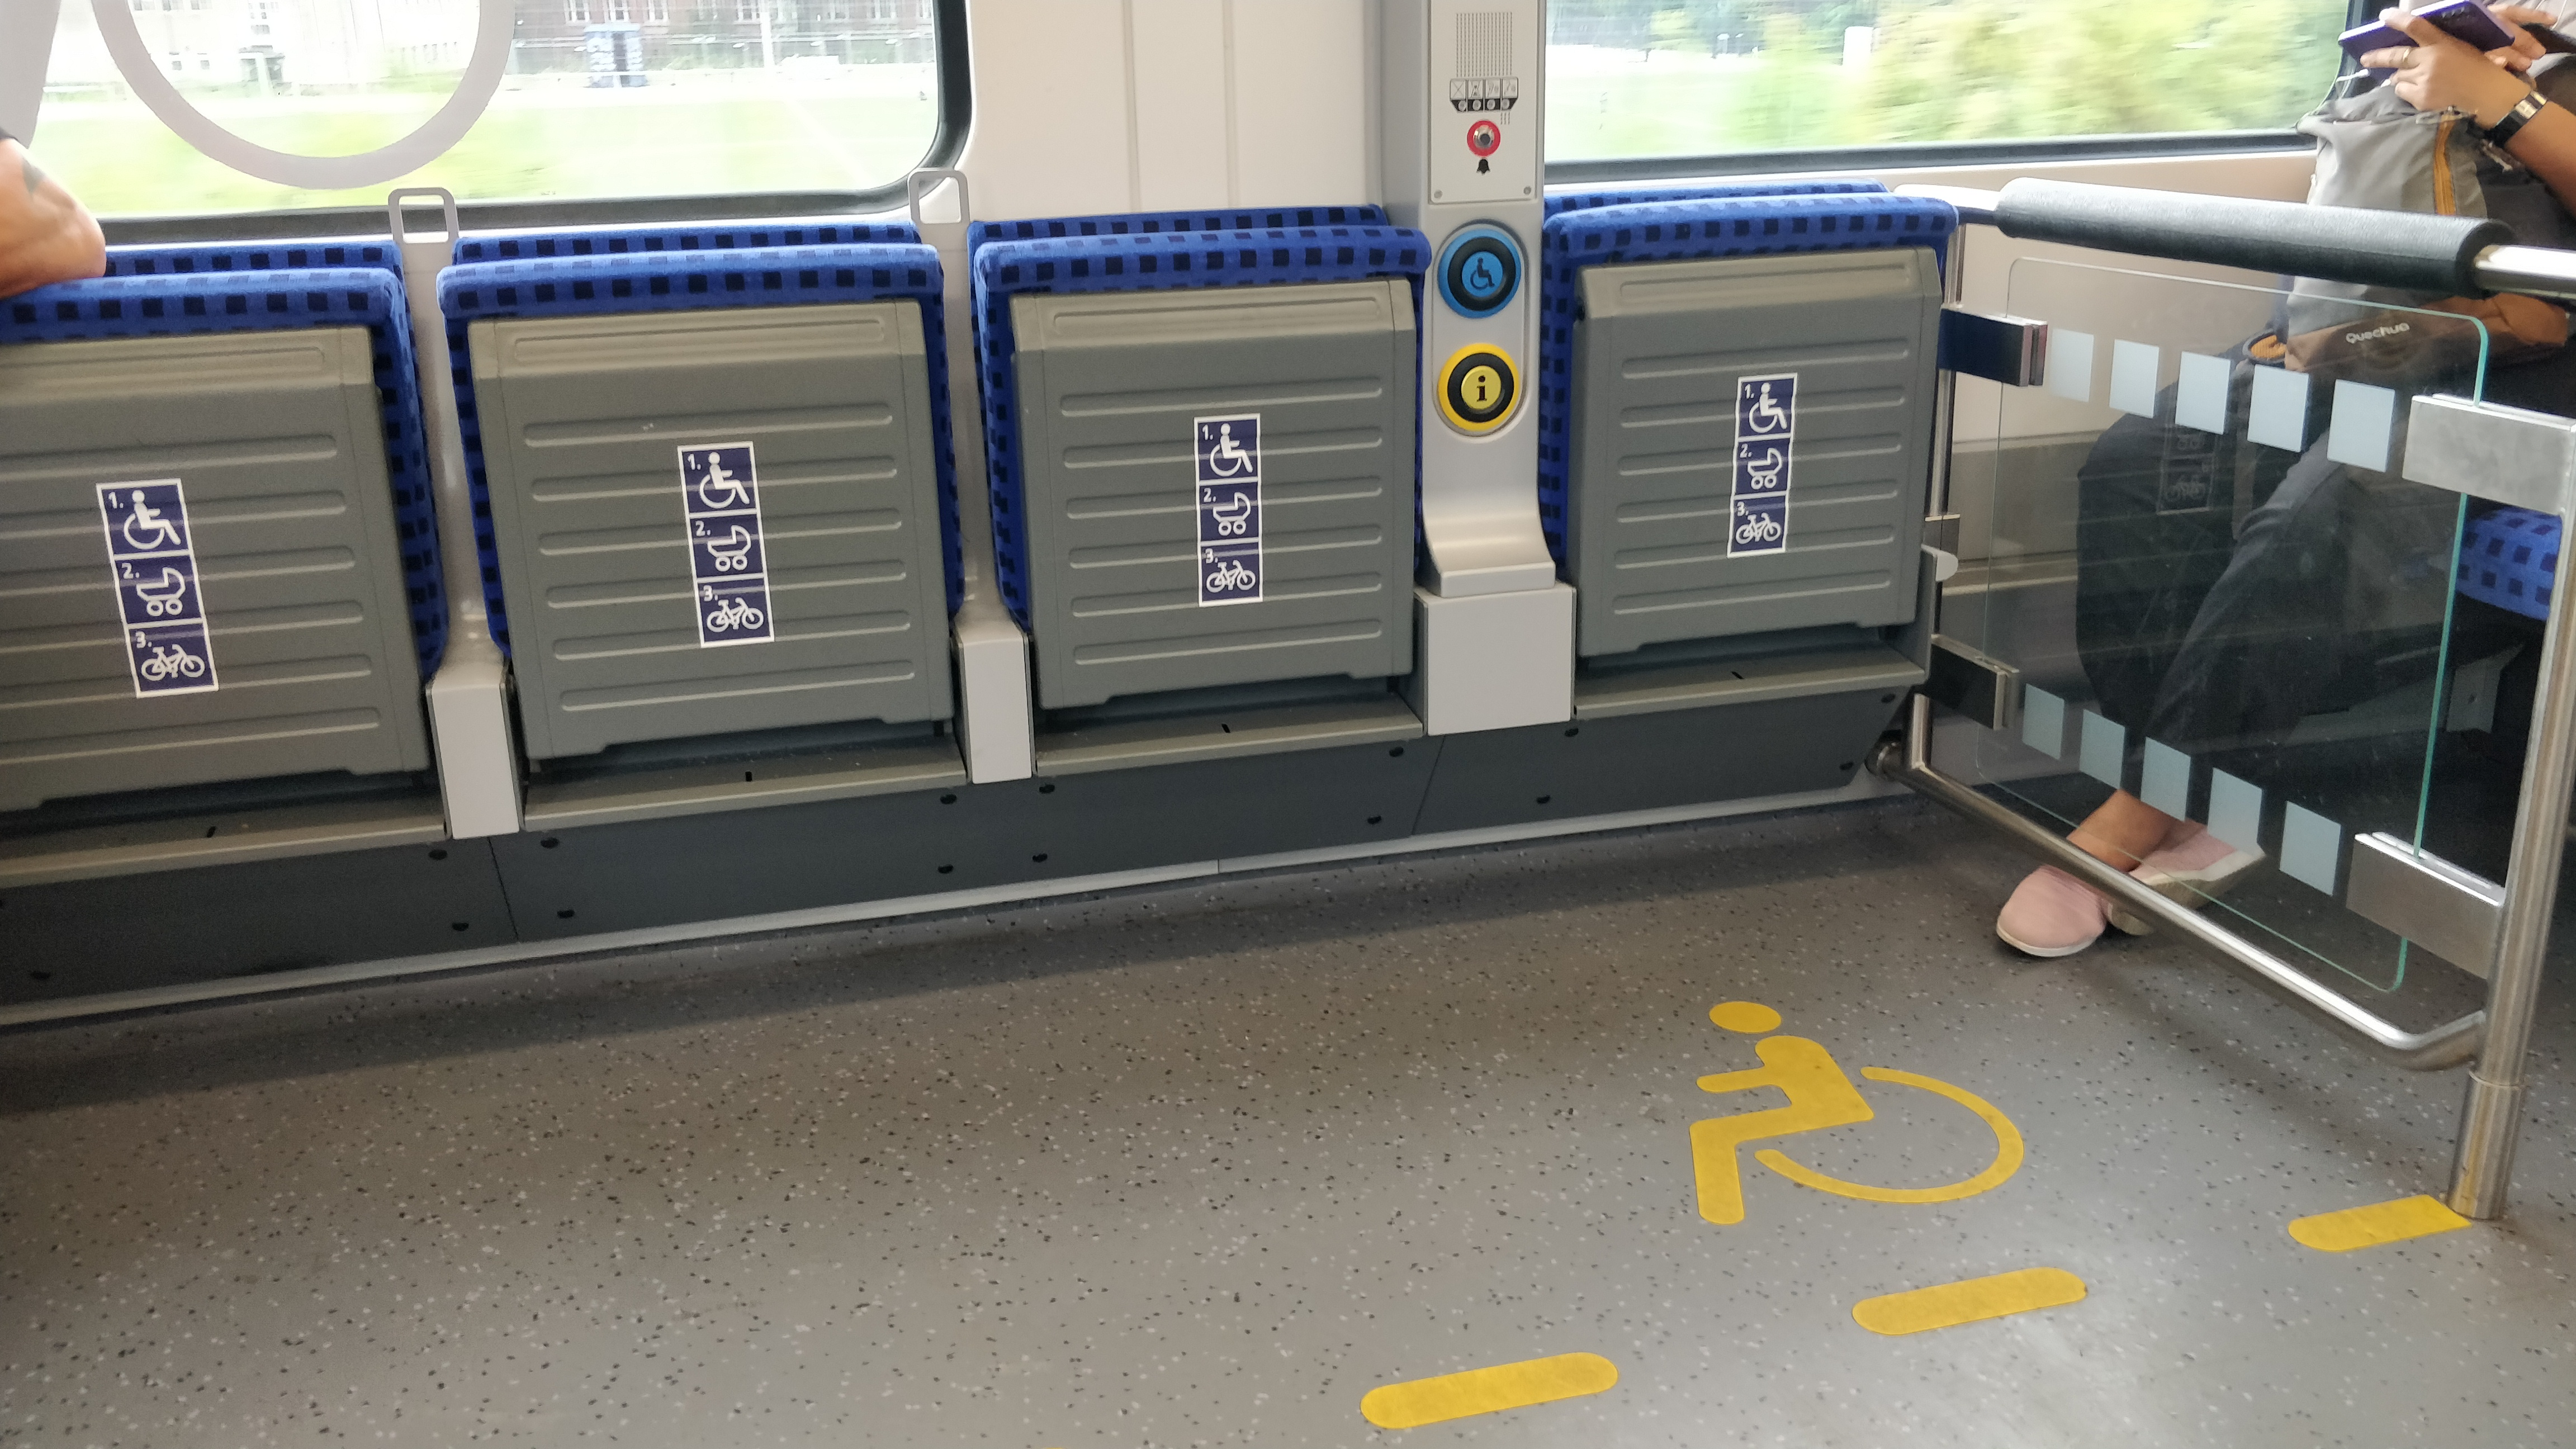
\includegraphics[width=0.7\textwidth]{images/IMG_20230826_102932-seats.jpg}
  \caption{Des sièges pliants et polyvalents à bord d'un train
    allemand, avec des indications de priorité pour les PMR, les mères
    avec jeunes enfants et les vélos.  Rien ne nous empêche de
    proposer la même chose en car.}
  \label{fig:train-velo-allemand-horizontal}
\end{figure}

Les espaces dédiés à ces vélos devraient être polyvalents (voir
figure~\ref{fig:train-velo-allemand-horizontal}) : des sièges pliants
permettraient, par exemple, de favoriser aussi bien les cyclistes que
les personnes à mobilité réduite, les femmes enceintes et l'ensemble
des usagers.

En adaptant nos TER et nos cars à la réalité multifacette du vélo
comme élément clé de la mobilité et en promouvant une intégration
harmonieuse entre le vélo et le train et car, avec accès sans barrière
et rangement horizontal, nous jetons les bases d'un système de
transport innovant et inclusif pour le futur.

\chapter{Structure de la métropole}

Pour rendre nos villes plus vivables, fluides et écologiques, il ne
suffit pas seulement de repenser nos modes de transport, mais aussi de
revoir la structure même de nos espaces urbains. Dans ce chapitre,
nous aborderons trois aspects essentiels de l'infrastructure
métropolitaine : la conception des carrefours, la gestion du
stationnement et la maintenance des voies.


\section{Poids lourds et carrefours}

Les poids lourds jouent un rôle central dans notre tissu économique,
garantissant la livraison de marchandises et le réapprovisionnement de
nos magasins. Toutefois, leur présence omniprésente façonne également
notre réseau routier, avec des aménagements tels que des voies larges
et des rayons de braquage étendus. Malheureusement, cette
infrastructure, bien qu'elle soit adaptée aux besoins des véhicules
lourds, peut compromettre la sécurité des piétons et des cyclistes.

En effet, la cohabitation sur nos rues entre ces mastodontes roulants
et les cyclistes ou piétons expose ces derniers à des risques
accrus. Alors, comment pouvons-nous protéger les usagers de la route
les plus vulnérables tout en assurant un transport efficace des
marchandises?

Il est essentiel d'envisager, sur le long terme, la réduction
progressive du recours aux poids lourds en milieu urbain. Pour ce
faire, repenser l'aménagement de nos rues est une première étape
cruciale. Dans ce contexte, l'adoption de solutions telles que les
palettes autonomes et les vélos cargo (pour les charges plus petites)
se présente comme une alternative pertinente. Non seulement ces
options offrent un moyen de transport de marchandises plus respectueux
de l'environnement, mais elles contribuent également à une meilleure
fluidité du trafic et à la diminution des congestions.

En adoptant une vision novatrice et en plaçant la sécurité et la
durabilité au cœur de nos politiques de transport, nous pouvons
transformer nos villes et nos régions en espaces plus verts, plus
sécurisés et plus agréables pour tous.

\refs

\begin{itemize}
\item \link{https://www.supplychaininfo.eu/vehicule-livraison-autonome/}
\item \link{https://www.groupestarservice.com/blog/vehicule-livraison-autonome/}
\item \link{https://www.zieglergroup.com/post/fr/pourquoi-le-groupe-ziegler-introduit-des-vehicules-de-livraison-autonomes-en-europe/}
\item \link{https://www.autoplus.fr/environnement/nuro-vehicule-autonome-livraison-552959.html\#item=1}
\item \link{https://www.usine-digitale.fr/article/nuro-presente-sa-troisieme-generation-de-robot-autonome-de-livraison.N1175542}
\item \link{https://adameo.com/blog/vehicule-autonome-et-transport-routier/}
\item \link{https://www.paris.fr/pages/logistique-marchandises-livraisons-4738}
\item \link{https://cdn.paris.fr/paris/2019/07/24/4cdaf0a5ab115898137e9093da69ae36.pdf}
\item \link{https://cdn.paris.fr/paris/2022/10/03/1bddb96a70a5b8df92b3258433fc83c3.pdf}
\item \link{https://www.paris.fr/pages/comment-paris-veut-repenser-sa-logistique-urbaine-21381}
\end{itemize}


\section{Services urbains}

Au fil du temps, nos villes se sont adaptées à accueillir les
véhicules lourds, ouvrant la voie aux services essentiels tels que les
pompiers et la collecte des déchets qui se servent presque uniquement
avec des véhicules lourds. Cependant, ces adaptations ont également
créé des barrières aux modes de transport plus écologiques et centrés
sur l'humain, comme la marche et le cyclisme. Alors que nous
envisageons un avenir où les rues sont plus accueillantes pour les
humains, nous devons également repenser la manière dont ces services
essentiels sont fournis.

Nous pouvons réduire la dépendance aux poids lourds tout en maintenant
des services essentiels efficaces et accessibles.  Il s'agit de penser
au remplacement avec du matériel plus adapté au fur et à mesure que
nous mettons à jour naturellement les véhicules de service actuels.

Nous offrons quelques exemples :

\textbf{Freiburg, Allemagne: Le modèle des "Vauban".}
Le quartier Vauban à Fribourg est une référence en matière de
conception urbaine écologique. Ici, la plupart des rues sont conçues
comme des "zones de rencontre", où les piétons et les cyclistes ont la
priorité. Pour résoudre la question des services d'urgence et de la
collecte des déchets, la ville a introduit des points de collecte
centralisés pour les déchets, éliminant ainsi le besoin de camions
poubelles pour naviguer dans de petites rues. Les services d'urgence
utilisent également des véhicules plus petits et plus agiles adaptés
aux rues étroites du quartier.

\textbf{Barcelone, Espagne: superblocks (superilles).}
Barcelone a commencé à mettre en œuvre le concept de "superblocks", de
grandes zones où la circulation est limitée et où les espaces sont
principalement réservés aux piétons et aux cyclistes. Pour la
prestation de services, des itinéraires spécifiques sont conçus pour
que les véhicules de service puissent accéder aux bâtiments sans
perturber la tranquillité des zones piétonnières. Ces routes spéciales
sont utilisées pour les services essentiels comme les pompiers et la
collecte des déchets.

\textbf{Ghent, Belgique: plan de circulation.}
Gand a mis en place un plan audacieux qui divise la ville en six zones
distinctes, accessibles uniquement par des routes périphériques. À
l'intérieur de ces zones, la priorité est donnée aux piétons, aux
cyclistes et aux transports en commun. Pour les services municipaux,
des véhicules plus compacts et écoénergétiques ont été adoptés. De
plus, les services de collecte de déchets encouragent le tri sélectif,
ce qui réduit le volume et la fréquence des ramassages.


\section{Abandonner l'exigence de création de places de parking}

Dans cette section, nous interrogeons l'obligation historique de créer
des places de stationnement voiture au sein des communes. Dans une
optique de mobilité durable à Nantes et dans les Pays de la Loire sur
les 25 années à venir, il est impératif de reconsidérer cette
pratique.

L'existence de places de stationnement voiture stimule l'usage de la
voiture individuelle. En offrant un espace privé pour le
stationnement, on incite à posséder une voiture. Ceci va à l'encontre
de nos ambitions de privilégier des moyens de transport
éco-responsables tels que les transports en commun, la marche ou le
vélo.

De plus, intégrer des places de stationnement dans les projets
immobiliers alourdit les coûts. Un parking souterrain peut coûter
entre 30 000 € à 50 000 € par emplacement, augmentant ainsi le coût
des logements. Ces frais viennent s'ajouter au prix de revient des
nouveaux logements, rendant ainsi l'accession à la propriété plus
onéreuse pour les citoyens.

Dans une perspective similaire, il convient d'encourager le citoyen
désireux de transformer de manière permanente son emplacement de
stationnement en un espace d'habitation, et ce, sans imposition de
frais.

Il est essentiel de repenser la systématisation des places de
stationnement dans les nouveaux projets urbains. Favorisons les
infrastructures qui réduisent la dépendance à la voiture. Cela
améliore la qualité de vie, diminue la congestion routière et préserve
l'environnement.

Il ne s'agit pas de proscrire totalement les places de stationnement,
mais de proscrire simplement l'obligation d'en créer. Les villes ayant
adopté cette approche ont constaté une réduction de près de 50~\% des
nouveaux emplacements créés.



\section{Repenser le stationnement commercial}

Pour une politique de transport durable, nous devons réviser notre
approche du stationnement commercial à Nantes et dans les Pays de la
Loire. Cette section traite des modifications nécessaires du code
municipal à ce sujet.

Au lieu de privilégier d'importants parkings en façade des magasins,
nous suggérons leur déplacement à l'arrière. Cette proposition
favorise l’expérience client, l'accessibilité et respecte
l'environnement. Repositionner les parkings transformera la perception
visuelle, mettant l'accent sur l'accès piétonnier et cycliste tout en
diminuant la dominance de l'automobile. Cela facilite également le
déplacement des clients entre commerces adjacents à pied. Le résultat
? Un commerce et un quartier qui valorisent les déplacements doux.

Par ailleurs, nous préconisons l'abolition de la contrainte de parking
pour les nouveaux commerces et ceux existants souhaitant
s'étendre. Cette liberté permettrait aux commerçants de réinventer
leurs espaces sans sacrifier de précieux mètres carrés pour le
stationnement voiture. Toutefois, nous ne sommes pas pour une
interdiction totale des parkings, mais nous croyons que c'est au
commerçant de définir le nombre de places adapté à ses besoins et à
son modèle économique.


\section{Travaux et restitution de la rue}

Lors de projets routiers entrepris par des entreprises privées, il est
primordial de veiller à une remise en état impeccable de la
chaussée. Cela assure non seulement la sécurité et le confort des
cyclistes, mais préserve également la longévité du revêtement. Les
chaussées mal restaurées se dégradent prématurément, engendrant des
coûts supplémentaires pour la métropole lors des nécessaires
interventions de resurfaçage.

La métropole se doit de garantir une supervision rigoureuse de ces
travaux. Elle pourrait également instaurer un système simplifié
permettant aux citoyens de signaler toute malfaçon sur la route. Cette
démarche collaborative, en impliquant les usagers, permettrait de
maintenir un niveau élevé de qualité de nos infrastructures routières.

Il s'agit là d'une question centrale pour la métropole. Au-delà du
confort des cyclistes, ces mesures sont également stratégiques du
point de vue financier. Un suivi rigoureux, appuyé par la vigilance
citoyenne, est essentiel pour une gestion durable et responsable de
notre réseau routier.

\section{Doux d’abord}

Lors de la conception de nouveaux espaces et quartiers urbains, un
changement radical de nos priorités en matière d'aménagement
s'impose. Notre proposition repose sur une approche claire et
résolument tournée vers l'avenir : mettre au premier plan la
conception des transports collectifs, suivis de près par les
déplacements piétonniers et cyclistes, et enfin, considérer
l'automobile.

Il ne s'agit pas de marginaliser l'automobile, mais de reconnaître une
réalité évidente : bien qu'essentielle, elle requiert une part
disproportionnée de notre espace urbain. Historiquement, nous avons
trop souvent adopté une stratégie axée sur la voiture, en reléguant
les transports collectifs, les infrastructures piétonnes et
éventuellement cyclables à une réflexion ultérieure, et souvent
marginale, justifiée par un prétendu manque d'espace.

Prenons l'exemple de l'Île de Nantes et du Quartier Mellinet : ces
zones, bien que récemment réaménagées, portent les marques d'une
planification priorisant excessivement l'automobile. L'espace,
idéalement destiné à promouvoir une mobilité douce et active, est
malheureusement dominé par des infrastructures orientées vers la
voiture. Si cette approche ne néglige pas totalement les espaces
verts, les zones piétonnes et les pistes cyclables sécurisées, elle
les relègue néanmoins à un second plan.

Pour envisager une mobilité durable, efficiente et respectueuse de
l'environnement à Nantes et dans les Pays de la Loire au cours des 25
prochaines années, nous devons adopter une vision rénovée de
l'aménagement urbain. C'est en redéfinissant nos priorités pour mettre
en avant les modes de transport éco-responsables et en concevant des
espaces urbains qui répondent aux aspirations modernes des citoyens
que nous parviendrons à une transformation profonde de notre mobilité.


\section{Réduction des îlots de chaleur urbains}

Les villes contemporaines, de par leur forte minéralisation,
contrastent avec les vastes étendues de prés et forêts qui les ont
précédées. Ce phénomène accentue la capacité des villes à capter la
radiation solaire et à la réémettre, jour comme nuit, créant ce que
l'on nomme des îlots de chaleur urbains (ICU). Ces ICU ne représentent
pas uniquement un enjeu de confort et de santé publique, mais
influencent également directement nos comportements de mobilité. En
effet, face à une température urbaine accablante, nombre de nos
concitoyens peuvent être tentés d'opter pour leurs véhicules
climatisés au détriment des transports collectifs, du vélo ou de la
marche.

Heureusement, la métropole dispose de plusieurs moyens économiques
pour combattre cet effet d'îlot de chaleur. Il est essentiel
d'atténuer l'absorption et l'émission de chaleur, tout en favorisant
les mécanismes naturels de rafraîchissement, tels que la circulation
de l'air et l'évapotranspiration.

Une première solution consiste à revisiter notre code d'urbanisme pour
encourager l'adoption de toitures réfléchissantes. Les modifications
apportées aux fenêtres pour réduire leur absorption thermique, ainsi
que l'intégration de panneaux solaires capables de transformer
l'énergie sans générer de chaleur, sont également des voies
prometteuses. Concernant les voies de circulation, typiquement
construites d'un mélange de goudron et de pierres concassées (macadam,
tarmac), l'utilisation de pierres plus claires pourrait réduire leur
capacité à retenir la chaleur.

Un autre axe d'intervention, d'égale importance, est la promotion de
la végétalisation urbaine. Les arbres, particulièrement efficaces pour
l'évapotranspiration, jouent un rôle central, mais même les petites
plantations urbaines contribuent au rafraîchissement de nos villes. Si
cette approche représente une solution économique, elle nécessite
cependant un engagement politique fort. En effet, l'espace dédié à
cette végétalisation se fera souvent au détriment de l'espace alloué à
la voiture. Cela souligne l'importance cruciale de l'ensemble des
mesures préconisées dans ce livre blanc pour une mobilité urbaine plus
durable et respectueuse de l'environnement.
\chapter{Fabrique social de la métropole}


\section{«~J'ai besoin de ma voiture~»}

«~J'ai besoin de ma voiture~» est une phrase fréquemment invoquée pour
justifier notre dépendance à l'automobile. Bien souvent, cette
affirmation reflète une réalité incontestable. Toutefois, elle nous
livre également un précieux indicateur que la métropole, les
départements et la région se doivent de prendre en considération. Il
est impératif de comprendre les contraintes qui rendent difficile le
passage à d'autres modes de transport et d'agir concrètement pour
faciliter cette transition.Il est tout aussi primordial que la
métropole communique de manière transparente et régulière sur les
initiatives mises en place et sur leur taux d'adoption. La réussite de
ces projets réside en grande partie dans la mobilisation et l'adhésion
des citoyens, à condition que ces projets soient clairement présentés
et justifiés.


\section{Le rôle singulier des écoles et des élèves}

Les enfants d'aujourd'hui façonnent le monde de demain. Leurs choix et
comportements influencent également ceux de leurs parents. Il est donc
primordial d'intégrer l'école, premier lieu de socialisation, dans nos
réflexions sur la mobilité de demain.

L'implication des jeunes ne doit pas être uniquement passive.  Nous
proposons de les engager dans l'évolution de leur propre mobilité, en
leur demandant de réfléchir et d'effectuer les changements.
Accompagnés par leur enseignants, nous suggérons que les écoliers
créent eux-même des jeux ou compétitions amiables (la
``gamification'') afin de s'encourager entre eux d'améliorer leur
propre mobilité.  Évidemment ils peuvent également réfléchir aux
incitations qui leur motiveraient les mieux.

Nous proposons en outre que les établissements scolaires publient
régulièrement en open data les modes de transport adoptés par leurs
élèves pour se rendre à l'école. Cela permettra de suivre et
d'encourager la proportion d'élèves optant pour des moyens de
déplacement écologiques.  Il ne s'agit pas d'instaurer un système de
surveillance lourd ni de mettre en place des pénalités, mais plutôt
d'établir un moyen transparent de suivre et encourager l'évolution des
habitudes de déplacement.

Bien que la métropole, le département et la région puissent définir
les grandes lignes des données à collecter, la mise en œuvre pourrait
être confiée aux acteurs locaux, y compris aux élèves eux-mêmes. Ces
derniers pourraient par exemple signaler leur mode de transport à leur
arrivée à l'école via une application mobile. Ou, dans un contexte
plus traditionnel, un enseignant pourrait simplement comptabiliser à
main levée les différents modes de transport. L'idée d'impliquer les
élèves dans la création d'un tel système, avec le soutien des
enseignants et administrateurs, est également une merveilleuse
opportunité pédagogique. L'essentiel est d'engager, de mesurer,
d'afficher et d'encourager une mobilité durable.

La publication régulière de ces données facilitera le dialogue entre
les différents acteurs – écoles, parents, élèves et élus. Ensemble,
ils pourront identifier des solutions pour encourager les modes de
déplacement non motorisés dans leurs quartiers.

Évidemment, un tel projet nécessiterait d'autres éléments : des
formations pour les enseignants sur la mobilité durable et les
avantages environnementaux et sociaux des modes de transport
écologiques.  Il serait judicieux également de sensibiliser les
parents pour qu'ils soutiennent leurs enfants dans ces choix.  Si les
écoles n'ont pas le matériel ou les infrastructures pour un transfert
modal des écoliers (abris et attaches vélo, par exemple, mais aussi
trottoirs et infrastructure cyclable autour des écoles), la métropole
doit être en mesure de participer à trouver des solutions rapides et
parfois tactiques, car un délai même de plusieurs années correspond à
un ``non'' absolu aux écoliers concernés.

Enfin, en intégrant les jeunes dans cette démarche, nous contribuerons
à changer leur perception des modes de transport. Il est crucial que
la nouvelle génération voie le choix d'alternatives écologiques non
pas comme une contrainte, mais comme une responsabilité et un
privilège. Trop souvent, la voiture est perçue comme un symbole de
maturité et d'indépendance. Il est temps de redéfinir ces aspirations
pour un avenir plus vert.

\chapter{Conclusions}

Dans ce livre blanc, nous avons détaillé les ambitions et projets
visant à transformer en profondeur la mobilité à Nantes Métropole et
dans les Pays de la Loire durant les 25 prochaines années. Cette durée
représente une opportunité majeure pour orienter, construire et guider
nos concitoyens vers une transition durable. L'objectif est clair :
établir un système de transport à la fois rentable, efficace et
respectueux de l'environnement. Cette mission s'ancre autour de
principes clés : transparence, clarté des objectifs et suivi des
avancées, tout en mettant en lumière les défis rencontrés.

Un premier axe d'action met l'accent sur la marche et le vélo. Cela
implique une refonte du stationnement, tant automobile que vélo, et
une révision des limites de vitesse. À moyen terme, éliminer les
obstacles verticaux devient impératif pour faciliter la mobilité de
tous, notamment les seniors, parents avec jeunes enfants et personnes
à mobilité réduite.

Le deuxième axe se concentre sur les transports en commun. Parmi les
solutions envisagées : intensifier la fréquence et l'amplitude des
services, remettre en service d'anciennes lignes et envisager des
services de cars express. Face à la congestion à la gare centrale de
Nantes, nous suggérons des mesures simples pour améliorer la fluidité
et la capacité.  De surcroît, nous soulignons l'importance d'une
meilleure accessibilité aux trains et cars. Le transport de vélos ne
doit plus être considéré comme une nécessité marginale réservée aux
sportifs, et l'accessibilité pour tous demeure une priorité.

Nous avons également souligné la nécessité de repenser
l'infrastructure de la métropole et de la région. Cela englobe la
réduction de la présence de véhicules lourds, l'adaptation de nos
véhicules de service à des rues conçues à l'échelle humaine, la
révision des obligations relatives à la construction de parkings, et
surtout, la priorisation des modes de transports actifs et doux dans
la conception urbaine, éliminant ainsi l'argument récurrent du "manque
d'espace".

Enfin, il est essentiel de tenir compte des signaux envoyés par nos
concitoyens quant à la nécessité de leurs voitures. La collaboration
avec les écoles et l'engagement des élèves sont cruciaux pour induire
une transformation culturelle durable.


\section*{À propos des Mobilitains}

Les Mobilitains, basées à Nantes Métropole, militent pour des
améliorations de la mobilité en région nantaise et dans les Pays de la
Loire.


\section*{Droit d'auteur}

Vous êtes autorisé à

\begin{itemize}
\item \textbf{Partager :} copier, distribuer et communiquer le
  matériel par tous moyens et sous tous formats.
\item \textbf{Adapter :}  remixer, transformer et créer à partir du
  matériel pour toute utilisation, y compris commerciale.
\end{itemize}

selon les conditions suivantes :

\begin{itemize}
\item \textbf{Attribution :} Vous devez créditer l'Œuvre, intégrer un
  lien vers la licence et indiquer si des modifications ont été
  effectuées à l'Oeuvre. Vous devez indiquer ces informations par tous
  les moyens raisonnables, sans toutefois suggérer que l'Offrant vous
  soutient ou soutient la façon dont vous avez utilisé son Oeuvre.
\item \textbf{Pas de restrictions complémentaires :} Vous n'êtes pas
  autorisé à appliquer des conditions légales ou des mesures
  techniques qui restreindraient légalement autrui à utiliser l'Oeuvre
  dans les conditions décrites par la licence.
\end{itemize}

\bigskip
{\small
\copyright{} Les Mobilitains,
CC BY-SA 4.0 \\
\url{https://creativecommons.org/licenses/by-sa/4.0/deed.fr}
}


\end{document}

